\documentclass[a4paper, portrait,12pt]{report}
\usepackage{palatino}
\renewcommand\familydefault{\sfdefault} 
\usepackage[verbose,a4paper,tmargin=2.5cm,bmargin=2.5cm,lmargin=2.5cm,rmargin=2.5cm]{geometry}
\usepackage[utf8]{inputenc}
\usepackage{polski}
\usepackage{amsmath}
\usepackage{amsfonts}
\usepackage{amssymb}
\usepackage{lastpage}
\usepackage{indentfirst}
\usepackage{float}
\usepackage{verbatim}
\usepackage{graphicx}
\usepackage{fancyhdr}
\usepackage{multirow}
\usepackage{array}
\usepackage{multicol}
\usepackage{tabu}
\usepackage{fancyhdr}
\usepackage{enumitem}
\pagestyle{fancy}
\frenchspacing
\pagestyle{fancyplain}
\fancyhf{}
\renewcommand{\headrulewidth}{0pt}
\renewcommand{\footrulewidth}{0.4pt}
\newcommand{\degree}{\ensuremath{^{\circ}}} 
\fancyhead[L]{WYDZIAŁ FIZYKI TECHNICZNEJ, INFORMATYKI i MATEMATYKI STOSOWANEJ \\
Instytut Fizyki PŁ}
\lhead{\small WYDZIAŁ FIZYKI TECHNICZNEJ, INFORMATYKI i MATEMATYKI STOSOWANEJ \\ Instytut Fizyki PŁ,}
\fancyfoot[C]{\thepage}
\renewcommand{\headrulewidth}{0.4pt}
\renewcommand{\footrulewidth}{0.4pt}
\newcolumntype{C}[1]{>{\centering\let\newline\\\arraybackslash\hspace{0pt}}m{#1}}
\setcounter{page}{1}
\usepackage{listings}
\usepackage{color}
\usepackage{pgfplots}
\usepgfplotslibrary{groupplots}
 \definecolor{codegreen}{rgb}{0,0.6,0}
\definecolor{codegray}{rgb}{0.5,0.5,0.5}
\definecolor{codepurple}{rgb}{0.58,0,0.82}
\definecolor{backcolour}{rgb}{0.95,0.95,0.92}
 
\lstdefinestyle{mystyle}{
    backgroundcolor=\color{backcolour},   
    commentstyle=\color{codegreen},
    keywordstyle=\color{magenta},
    numberstyle=\tiny\color{codegray},
    stringstyle=\color{codepurple},
    basicstyle=\footnotesize,
    breakatwhitespace=false,         
    breaklines=true,                 
    captionpos=b,                    
    keepspaces=true,                 
    numbers=left,                    
    numbersep=5pt,                  
    showspaces=false,                
    showstringspaces=false,
    showtabs=false,                  
    tabsize=2
}
 
\lstset{style=mystyle}


\usepackage{xcolor}
\lstset { %
    language=C++,
    backgroundcolor=\color{black!5}, % set backgroundcolor
    basicstyle=\footnotesize,% basic font setting
}


\begin{document}
\section{Laser 635\,nm}
\begin{table}
\begin{center}
\caption{ Wyznaczone wartośc prądu progowego $I_{\mathrm{th}}$ w różnych temperaturach $T$ dla lasera krawędziowego 635\,nm. }
\begin{tabular}{ | C{1.5cm}|  C{1.5cm} | C{1.5cm} | C{1.5cm}| C{1.5cm} | C{1.5cm}| C{1.5cm}| C{2.0cm}| C{2.0cm}|}
\hline
$T$ [K] 	&   278 & 283  	& 288 & 293 & 298 & 303 & 308 \\ \hline
$I_{\mathrm{th}}$ [mA]  &	19.1 $\pm$ 0.2  & 20.7 $\pm$ 0.2 & 22.6 $\pm$ 0.2 &
25.0 $\pm$ 0.2  & 27.9 $\pm$ 0.3 & 31.4 $\pm$ 0.5 & 36 $\pm$ 2	\\ \hline
\end{tabular}
\end{center}
\end{table}
%\begin{figure}
%\center
%  \includegraphics[scale=0.30]{plot635/plot_ivl_4.eps}
%  \label{rys1}
%  \caption{Wykres napięcia i mocy od prądu dla lasera krawędziowego 635\,nm.}
%\end{figure}
\begin{figure}
\center
  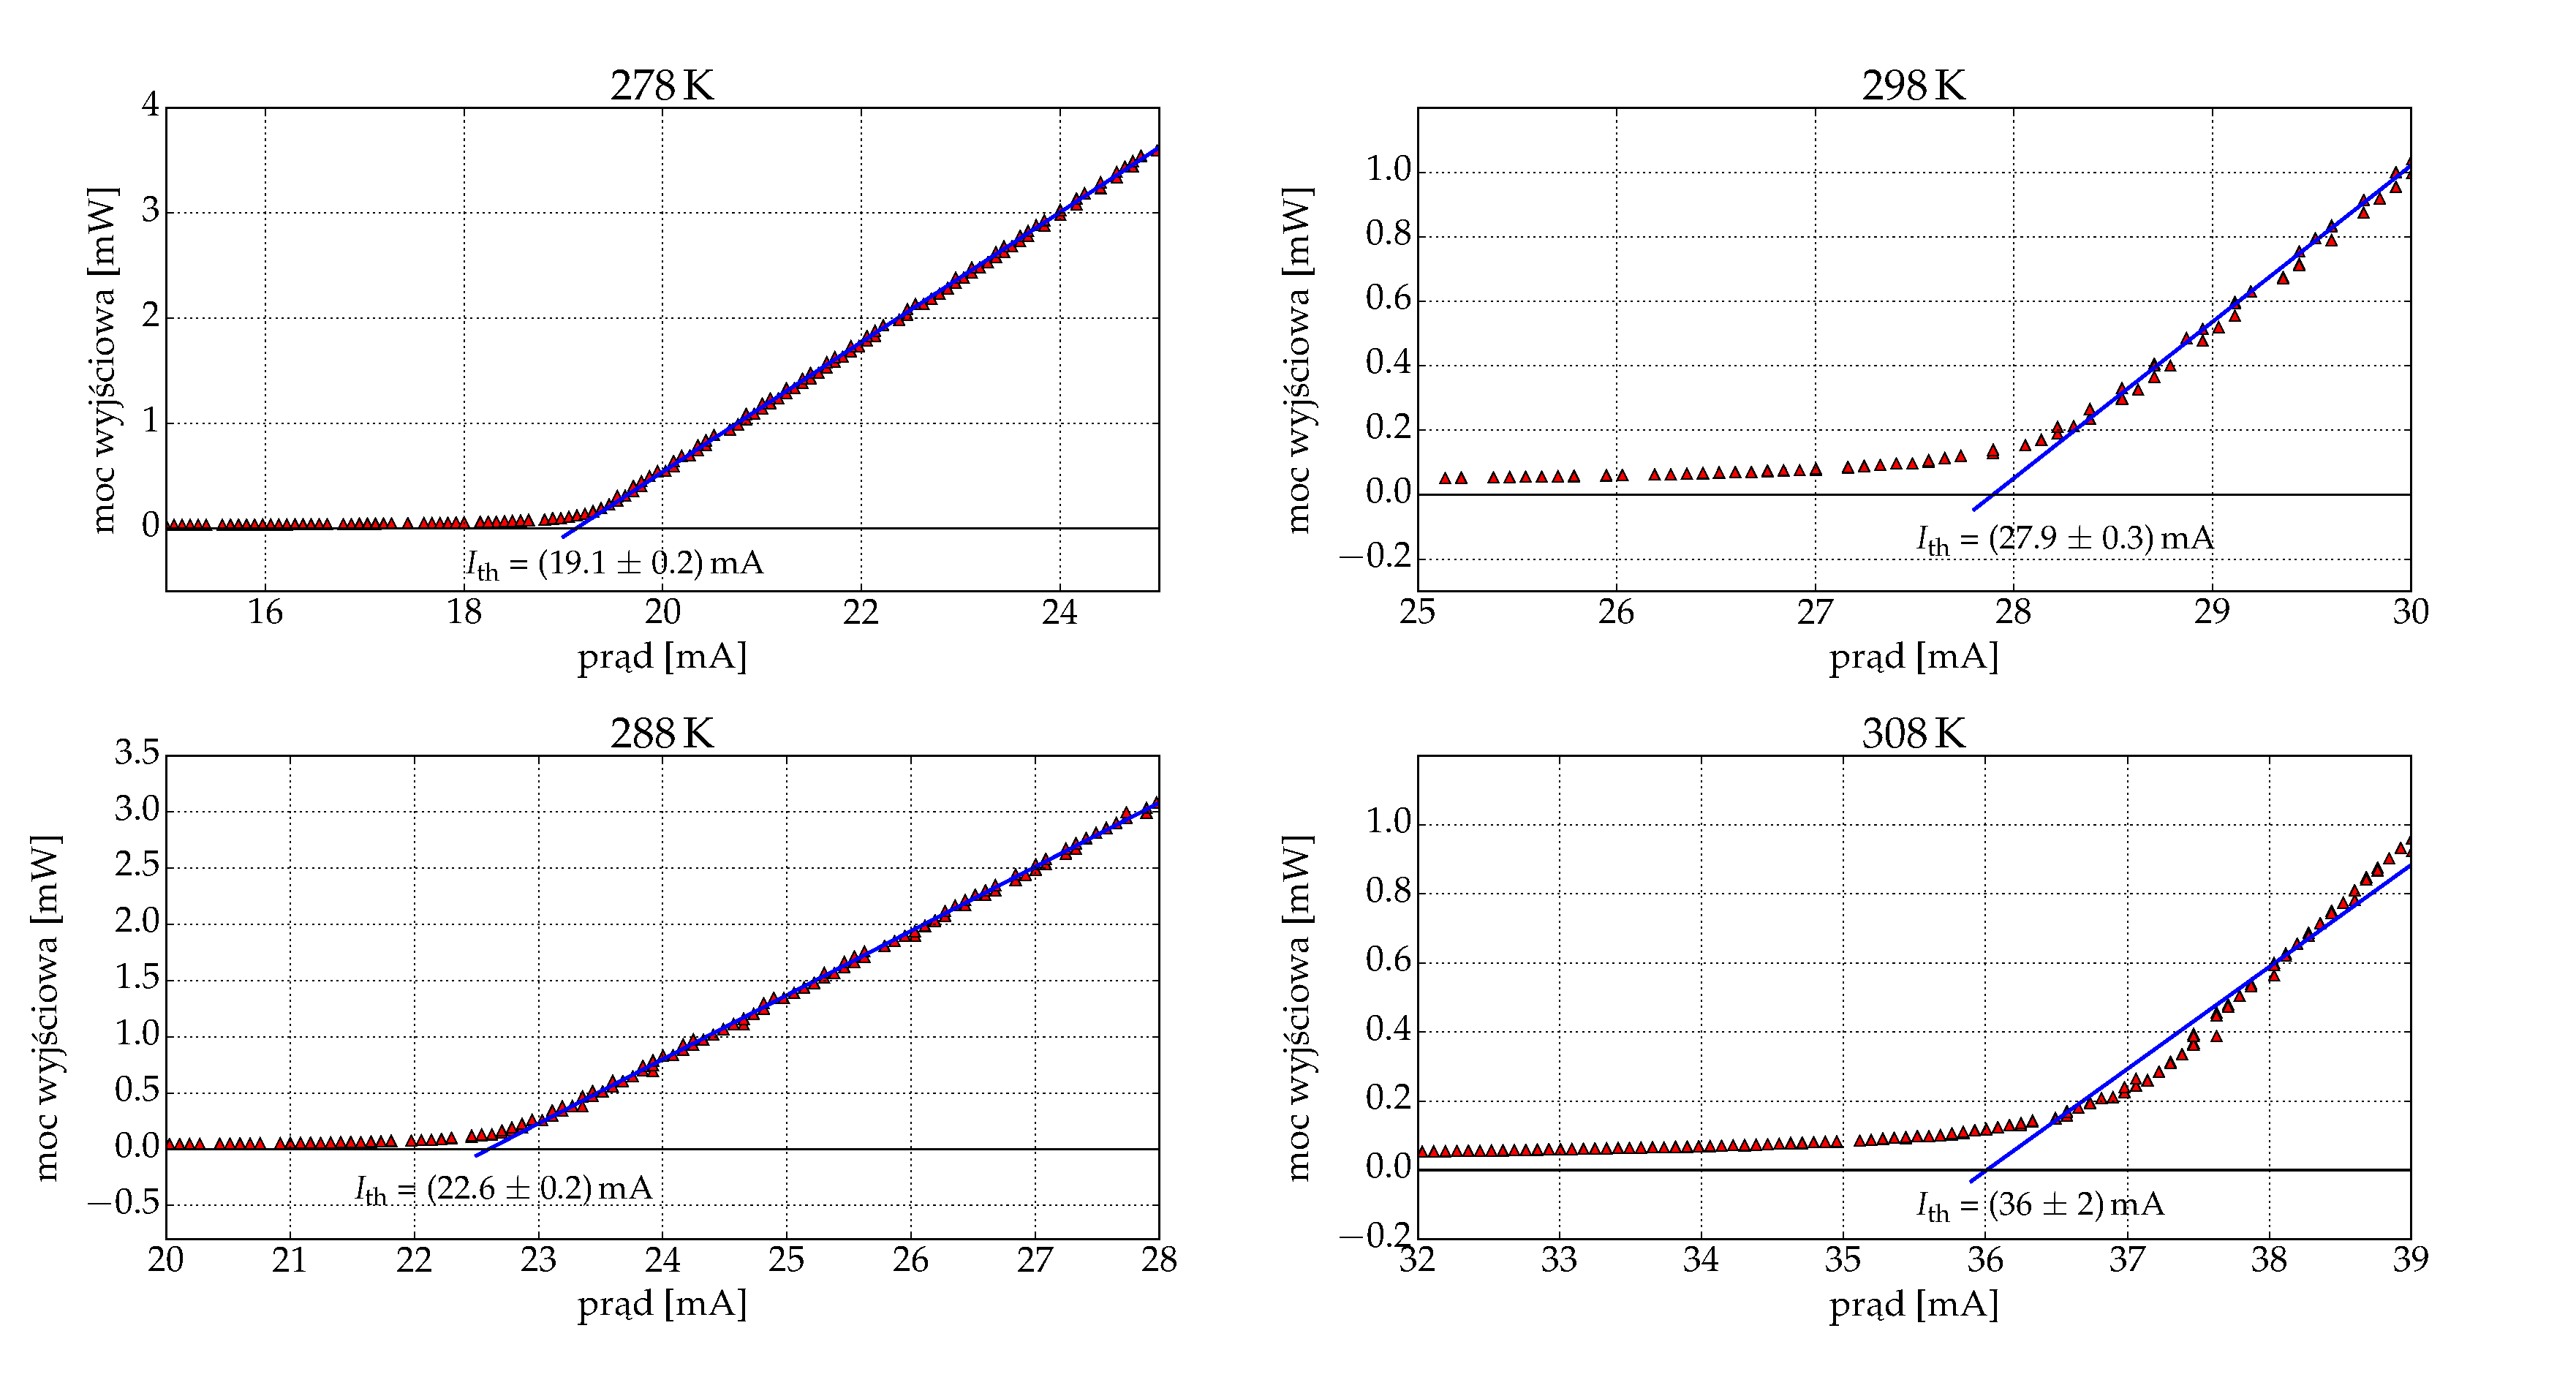
\includegraphics[scale=0.30]{plot635/plot_i_th_4.eps}
  \label{rys2}
  \caption{Wykres prądu progowego dla lasera krawędziowego 635\,nm.}
\end{figure}
\begin{figure}
\center
  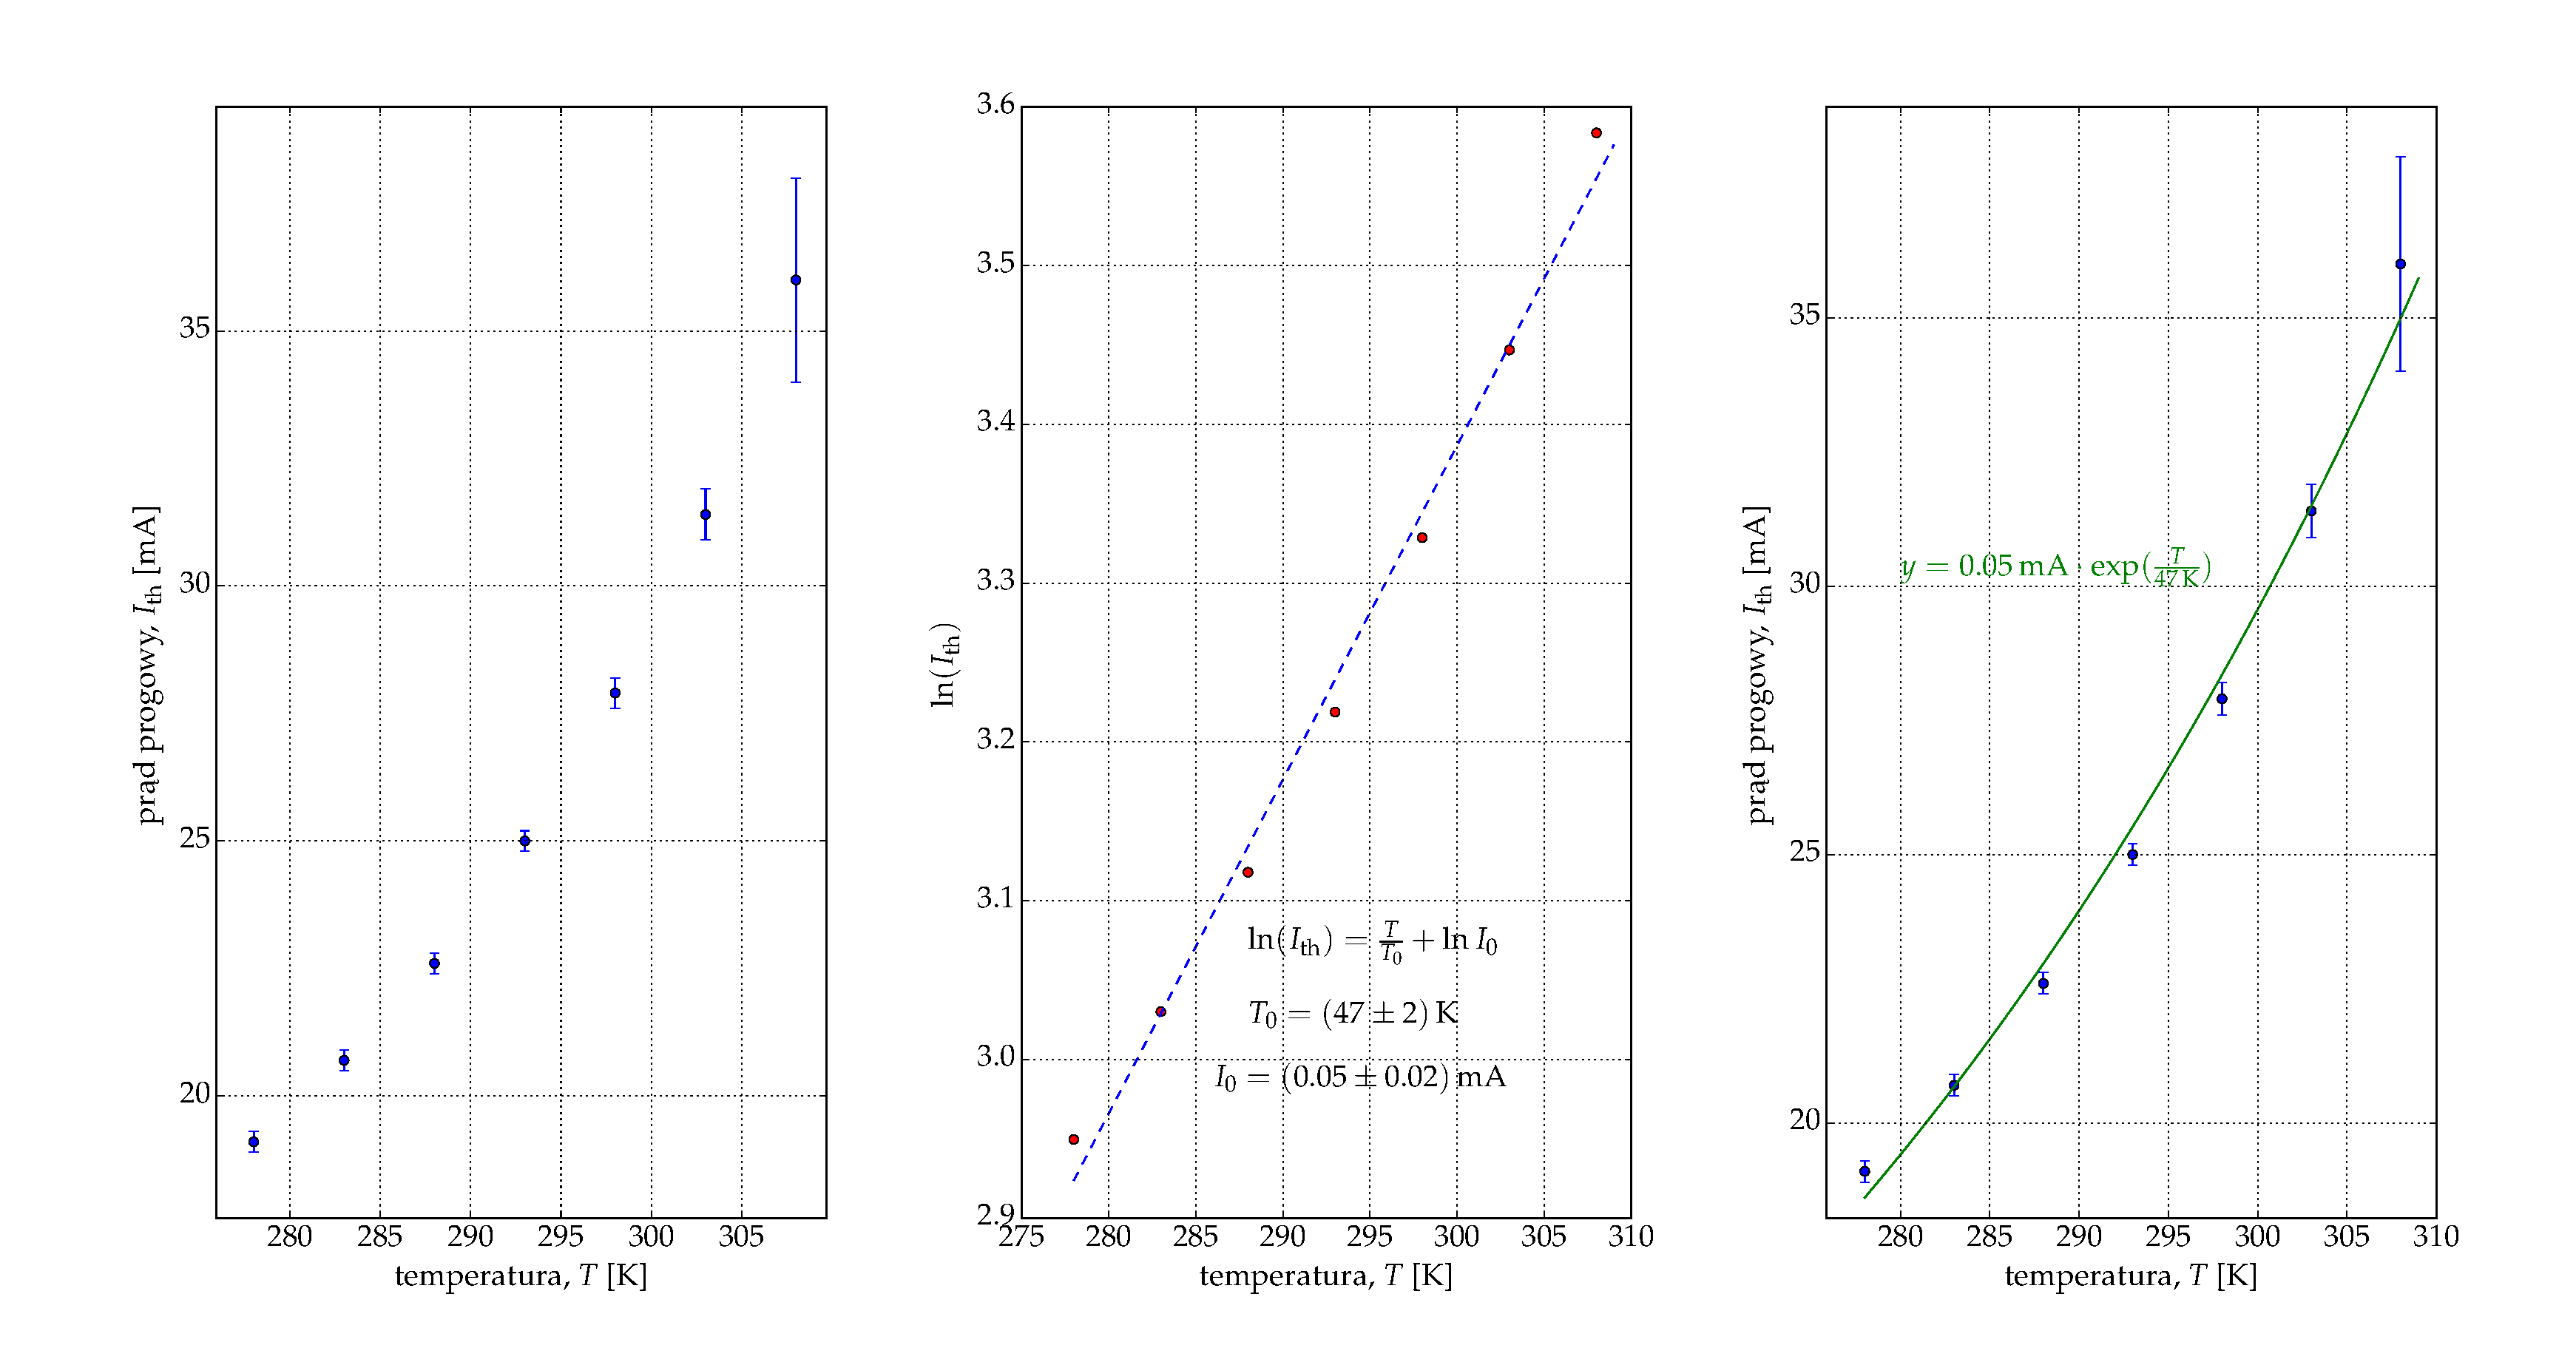
\includegraphics[scale=0.30]{plot635/plot_fit.eps}
  \label{rys2}
  \caption{Wykres prądu progowego z dopasowanymi wartościami $I_{0}$ i $T_{0}$ dla lasera krawędziowego 635\,nm.}
\end{figure}
\begin{figure}
\center
  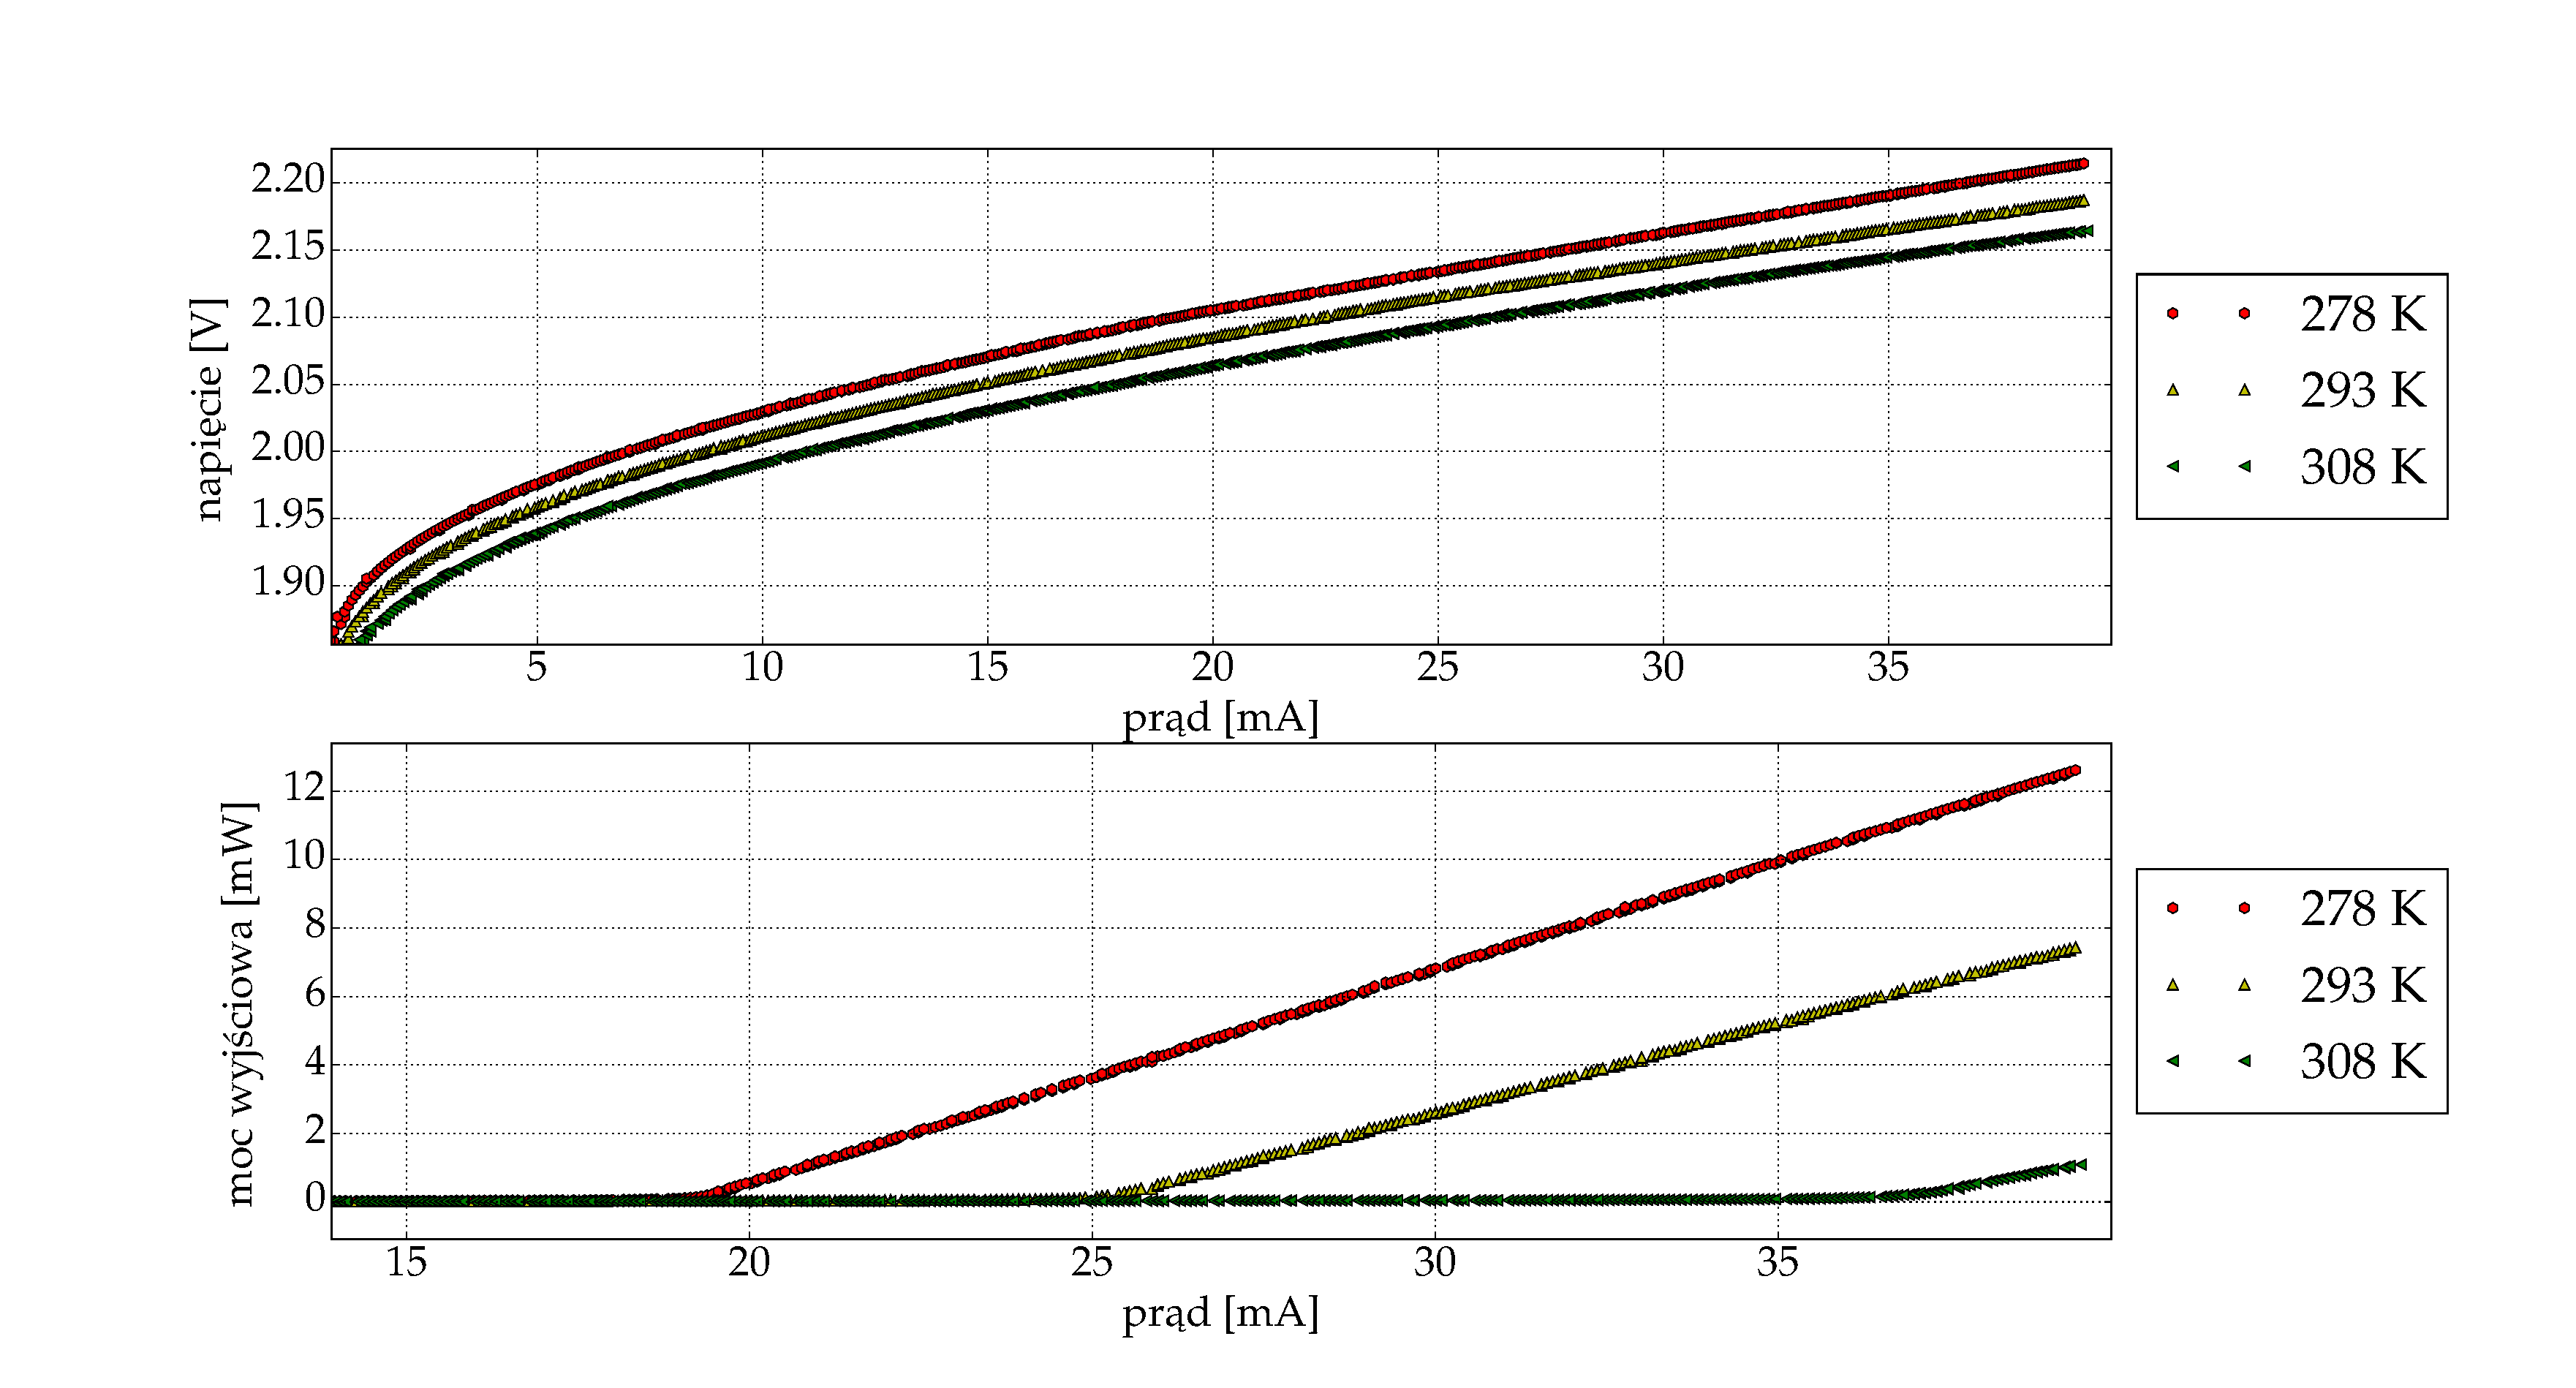
\includegraphics[scale=0.30]{plot635/plot_voltage_power.eps}
  \label{rys3}
  \caption{Wykres napięcia na laserze oraz mocy w funkcji prądu dla lasera krawędziowego 635\,nm.}
\end{figure}
\begin{figure}
\center
  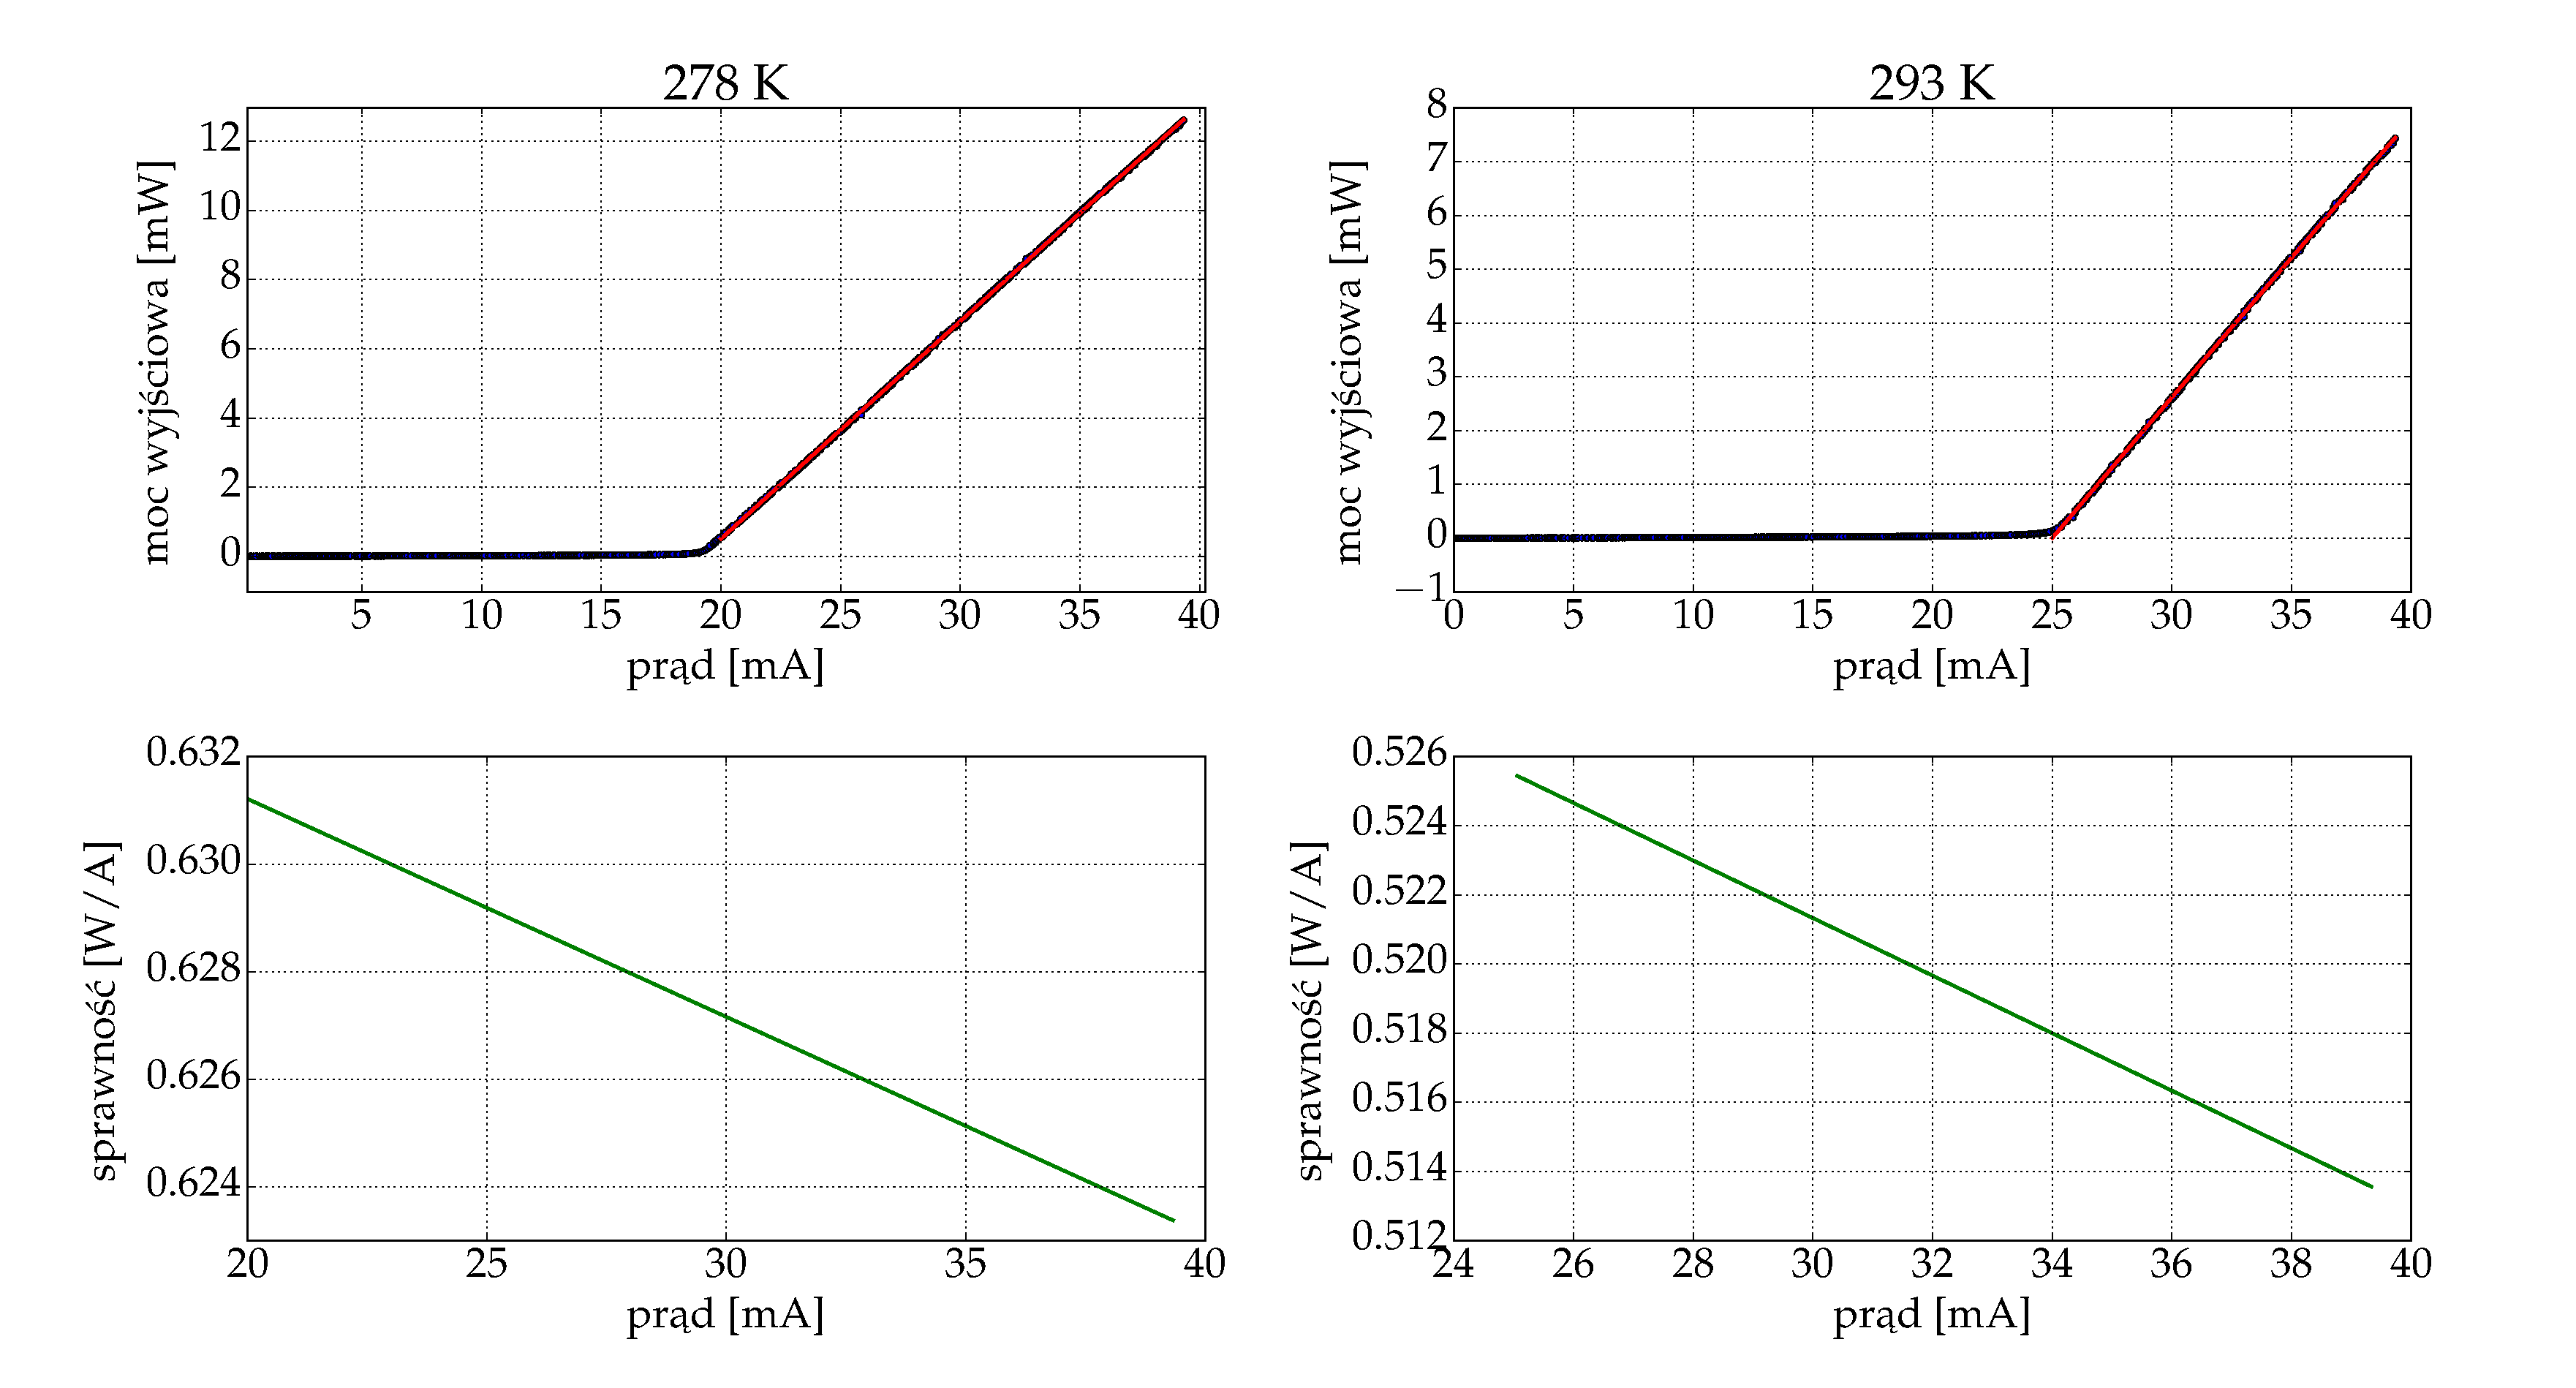
\includegraphics[scale=0.30]{plot635/plot_eff_via_current4.eps}
  \label{rys3}
  \caption{Wykres sprawności różniczkowej dla lasera krawędziowego 635\,nm dla dwóch temperatur.}
\end{figure}
\begin{figure}
\center
  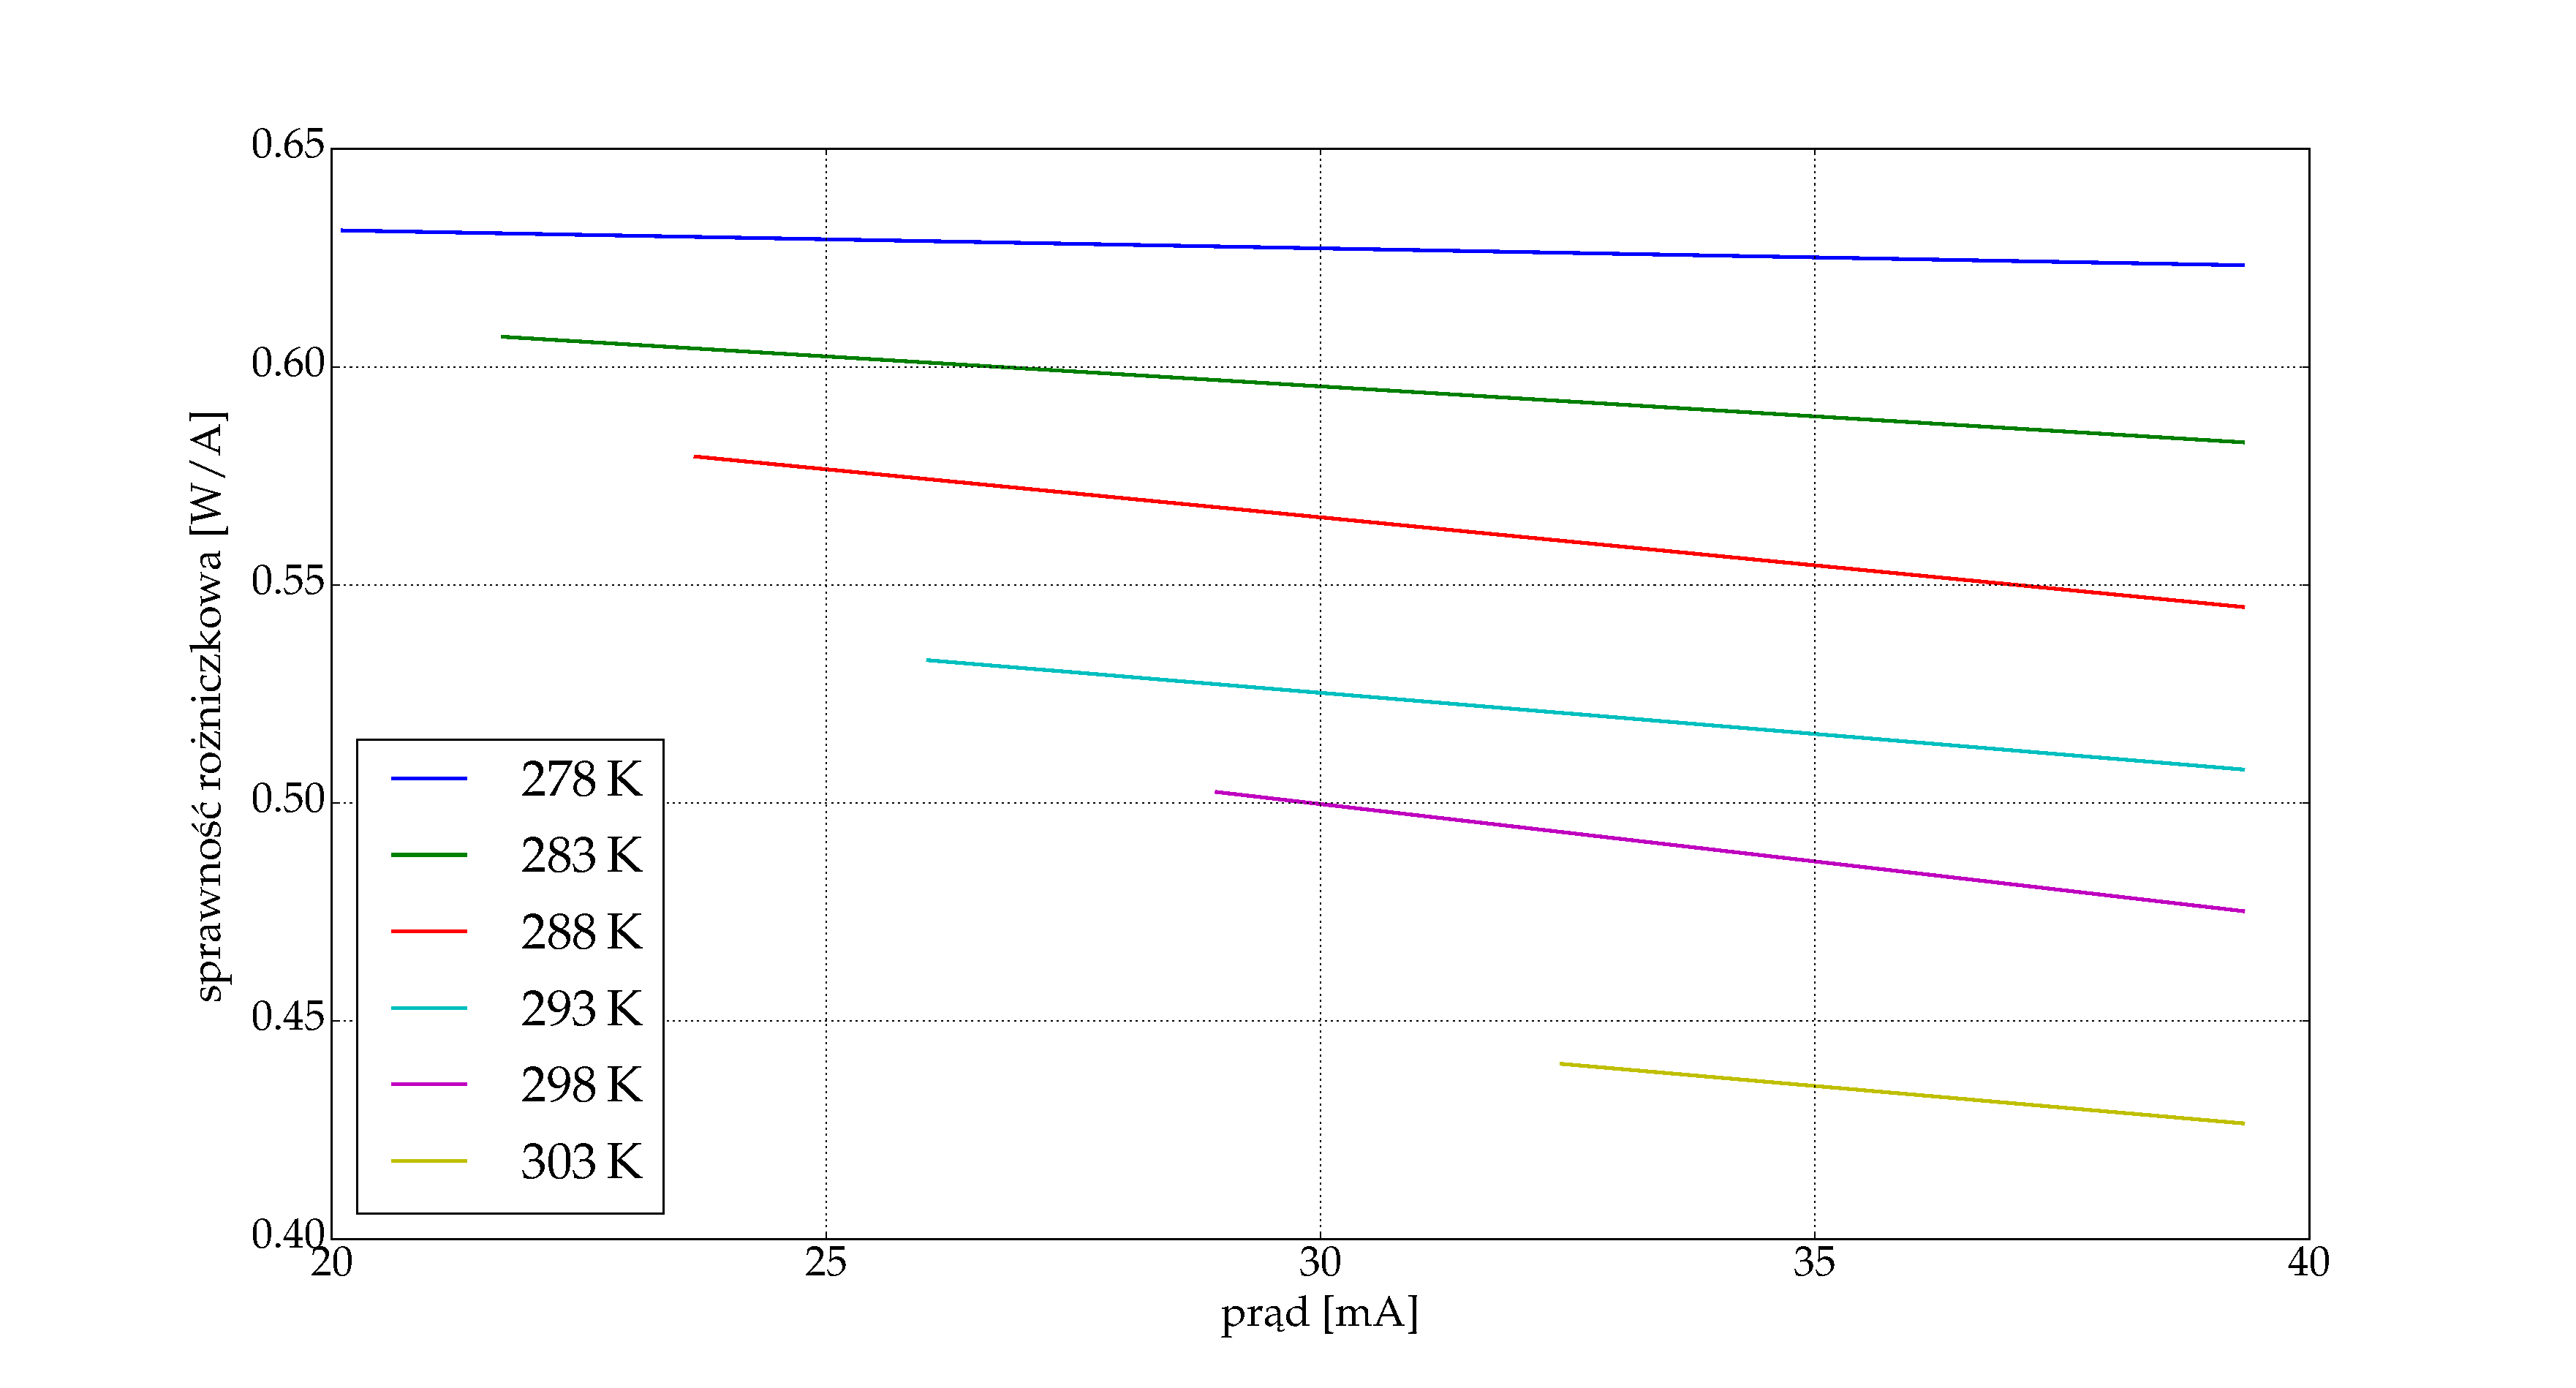
\includegraphics[scale=0.30]{plot635/plot_eff_via_current_all.eps}
  \label{rys3}
  \caption{Wykres sprawności w funkcji prądu dla lasera krawędziowego 635\,nm.}
\end{figure}
\newpage
\newpage
\subsection{Laser VCSEL 850\,nm --- omówienie wyników}
Pomiar przeprowadzany był w temperaturach chłodnicy od 283\,K do 353\,K, krokiem co 5\,K. Wartości wyznaczonego prądu progowego
znajdują się w tabeli~\ref{tab:tabela_vcsel850}. Rysunki od ~\ref{fig:plot_fit_i_th_vcsel850} do ~\ref{fig:plot_eff_all_via_current_vcsel850} dotyczą lasera
VCSEL 850\,nm.
\begin{itemize}
\item Wykres na rysunku~\ref{fig:plot_fit_i_th_vcsel850} przedstawia sposób wyznaczana wartość prądu progowego. Następnie na podstawie
wyznaczonych wartości w danej temperaturze, sporządziłem wykres prądu progowego w zależności od temperatury
przedstawiony na rysunku~\ref{fig:plot_temp_i_th_log_lin_vcsel850}. Jak widzimy, wykres ten charakteryzuje się pewnym minimum, które
osiągane jest w temperaturze 298\,K.
\item Analizując wykres napięcia na laserze od prądu wejściowego przedstawiony na rysunku~\ref{fig:plot_power_voltage_vcsel850}
można zauważyć, że wraz ze wzrostem temperatury na chłodnicy
maleje opór lasera. Wraz ze wzrostem temperatury chłodnicy maleje, także moc wyjściowa lasera.
\item Wykres na rysunku~\ref{fig:plot_eff_all_via_current2_vcsel850} przedstawia sprawność różniczkowa lasera w funkcji prądu wejściowego
od temperatury na chłodnicy. W górnej części rysunku pokazana jest zależność mocy wyjściowej od prądu, do której dopasowałem
funkcją kwadratowa dla punktów leżących powyżej wartości prądu progowego. Dopasowana funkcja zbliżona jest do funkcji kwadratowej,
przez co zmiany sprawności wraz ze wzrostem prądu jest dosyć duża.
\item Wykres na rysunku~\ref{fig:plot_eff_all_via_current_vcsel850} przedstawia jak, zmienia się sprawność lasera od temperatury chłodnicy.
Funkcje, które przedstawiają sprawność zostały wyznaczone analogicznie jak te przedstawione na rysunku~\ref{fig:plot_eff_all_via_current2_vcsel850}.
Analizując ten wykres, dochodzę do wniosku, że wraz z wyższą temperaturą sprawność lasera maleje.
\end{itemize}
\begin{table}[H]
\begin{center}
\caption{ Wyznaczone wartośc prądu progowego $I_{\mathrm{th}}$ w różnych temperaturach $T$ dla lasera VCSEL 850\,nm.}
\begin{tabular}{ | C{1.5cm}|  C{3.0cm} | C{1.5cm} | C{3.0cm}| C{1.5cm} | C{3.0cm}|}
\hline
$T$ [K] &   $I_{\mathrm{th}}$ [mA]  &  $T$ [K] &   $I_{\mathrm{th}}$ [mA]  &  $T$ [K] &   $I_{\mathrm{th}}$ [mA] 	\\ \hline
283      &   1.70 $\pm$ 0.03  & 288      &   1.67 $\pm$ 0.03   & 293		 &   1.60 $\pm$ 0.03  \\ \hline
298		 &   1.55 $\pm$ 0.04  & 303		 &   1.59 $\pm$ 0.03  & 308		 &   1.63 $\pm$ 0.03  \\ \hline
313		 &   1.65 $\pm$ 0.03  & 318		 &   1.68 $\pm$ 0.04  & 323		 &   1.73 $\pm$ 0.04  \\ \hline
328		 &   1.83 $\pm$ 0.04  & 333		 &   1.89 $\pm$ 0.04  & 338		 &   2.01 $\pm$ 0.04  \\ \hline
343		 &   2.14 $\pm$ 0.04  & 348		 &   2.24 $\pm$ 0.05  & 353		 &   2.38 $\pm$ 0.05  \\ \hline
358		 &   2.57 $\pm$ 0.05  & 363		 &   2.74 $\pm$ 0.07  \\ \cline{1-4}
\end{tabular}
\label{tab:tabela_vcsel850}
\end{center}
\end{table}
\begin{figure}[H]
\center
  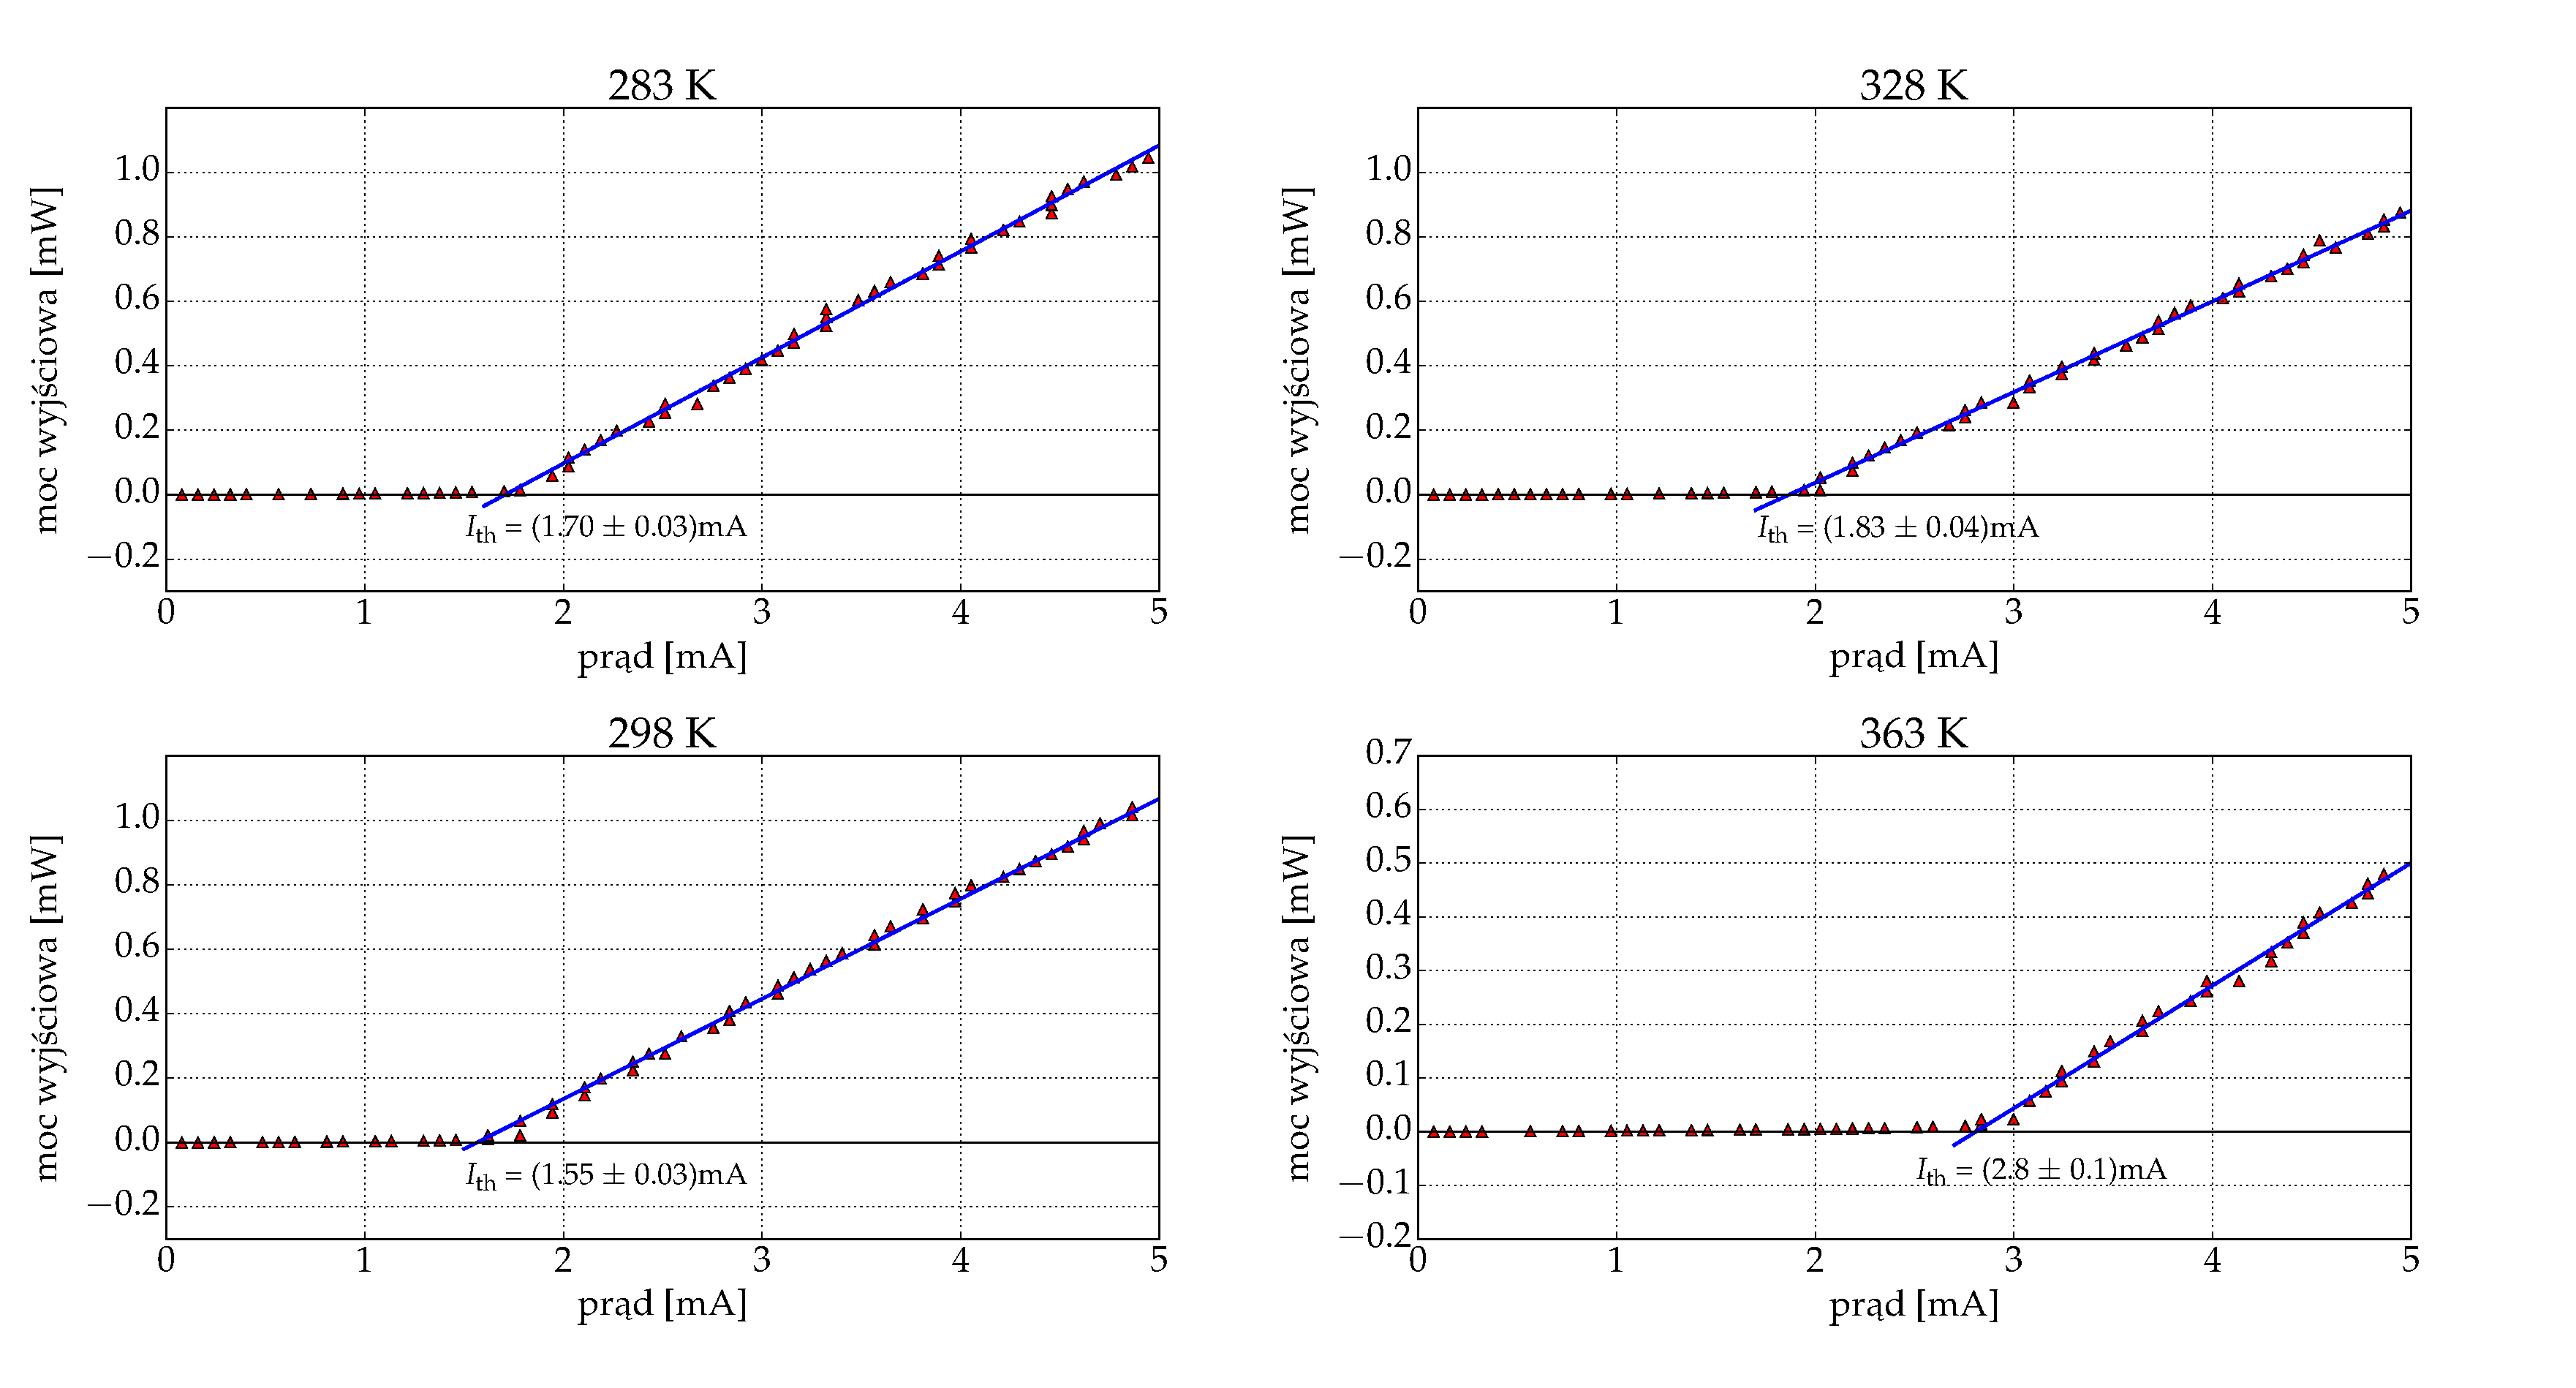
\includegraphics[scale=0.30]{plot_vcsel_850/plot_fit_i_th.eps}
  \caption{Wykres ilustrujący wyznaczanie prądu progowego dla lasera VCSEL 850\,nm.}
  \label{fig:plot_fit_i_th_vcsel850}
\end{figure}
\begin{figure}
\center
  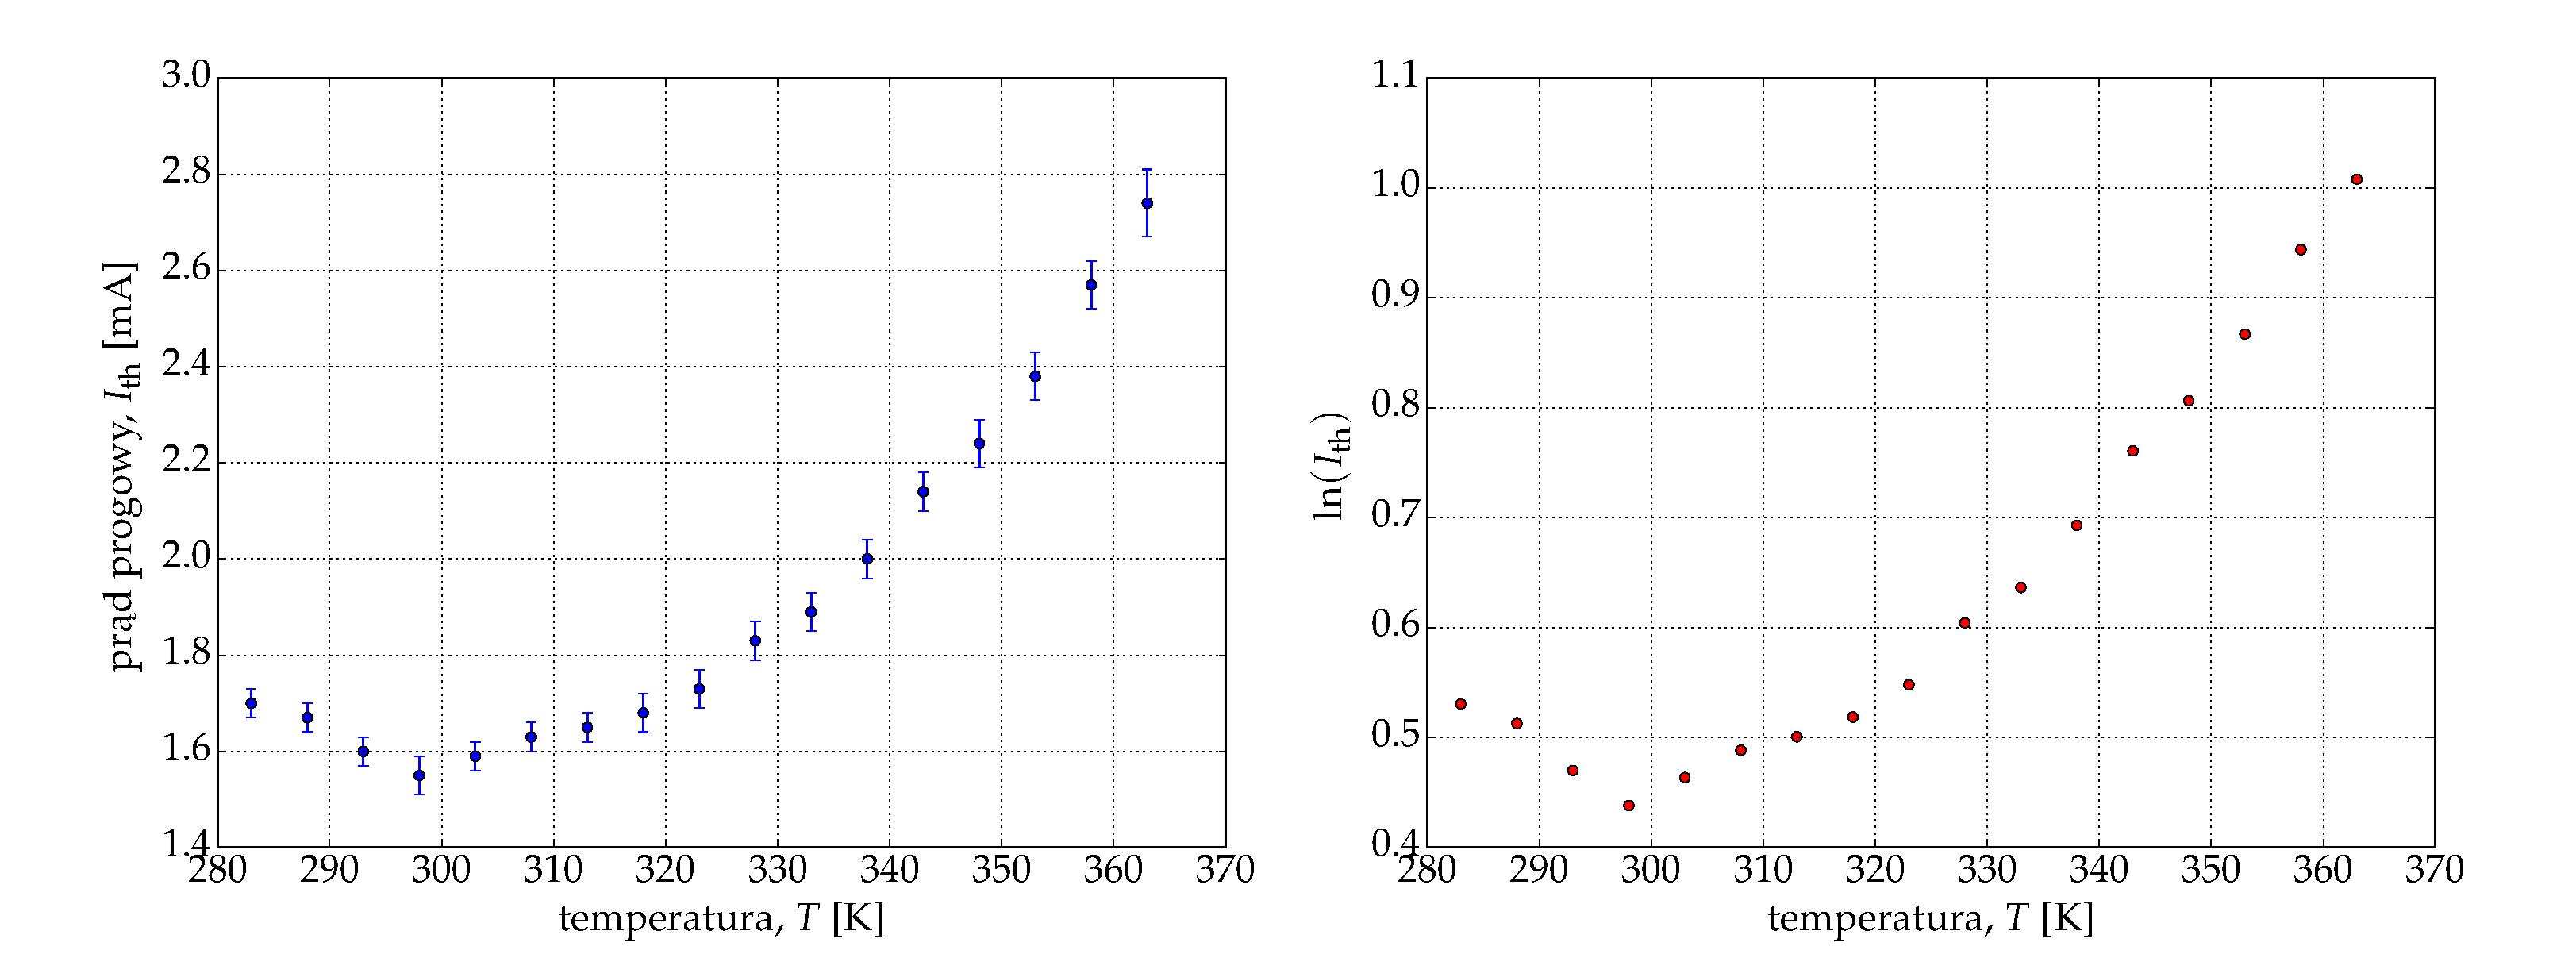
\includegraphics[scale=0.30]{plot_vcsel_850/plot_temp_i_th_log_lin.eps}
  \caption{Wykres prądu progowego od temperatury dla lasera VCSEL 850\,nm.}
  \label{fig:plot_temp_i_th_log_lin_vcsel850}
\end{figure}
%\begin{figure}
%\center
%  \includegraphics[scale=0.30]{plot_vcsel_850/plot_ivl_4.eps}
%  \caption{Sprawność VCSEL 850.}
%  \label{vcsel_850_rys_1}
%\end{figure}
\begin{figure}
\center
  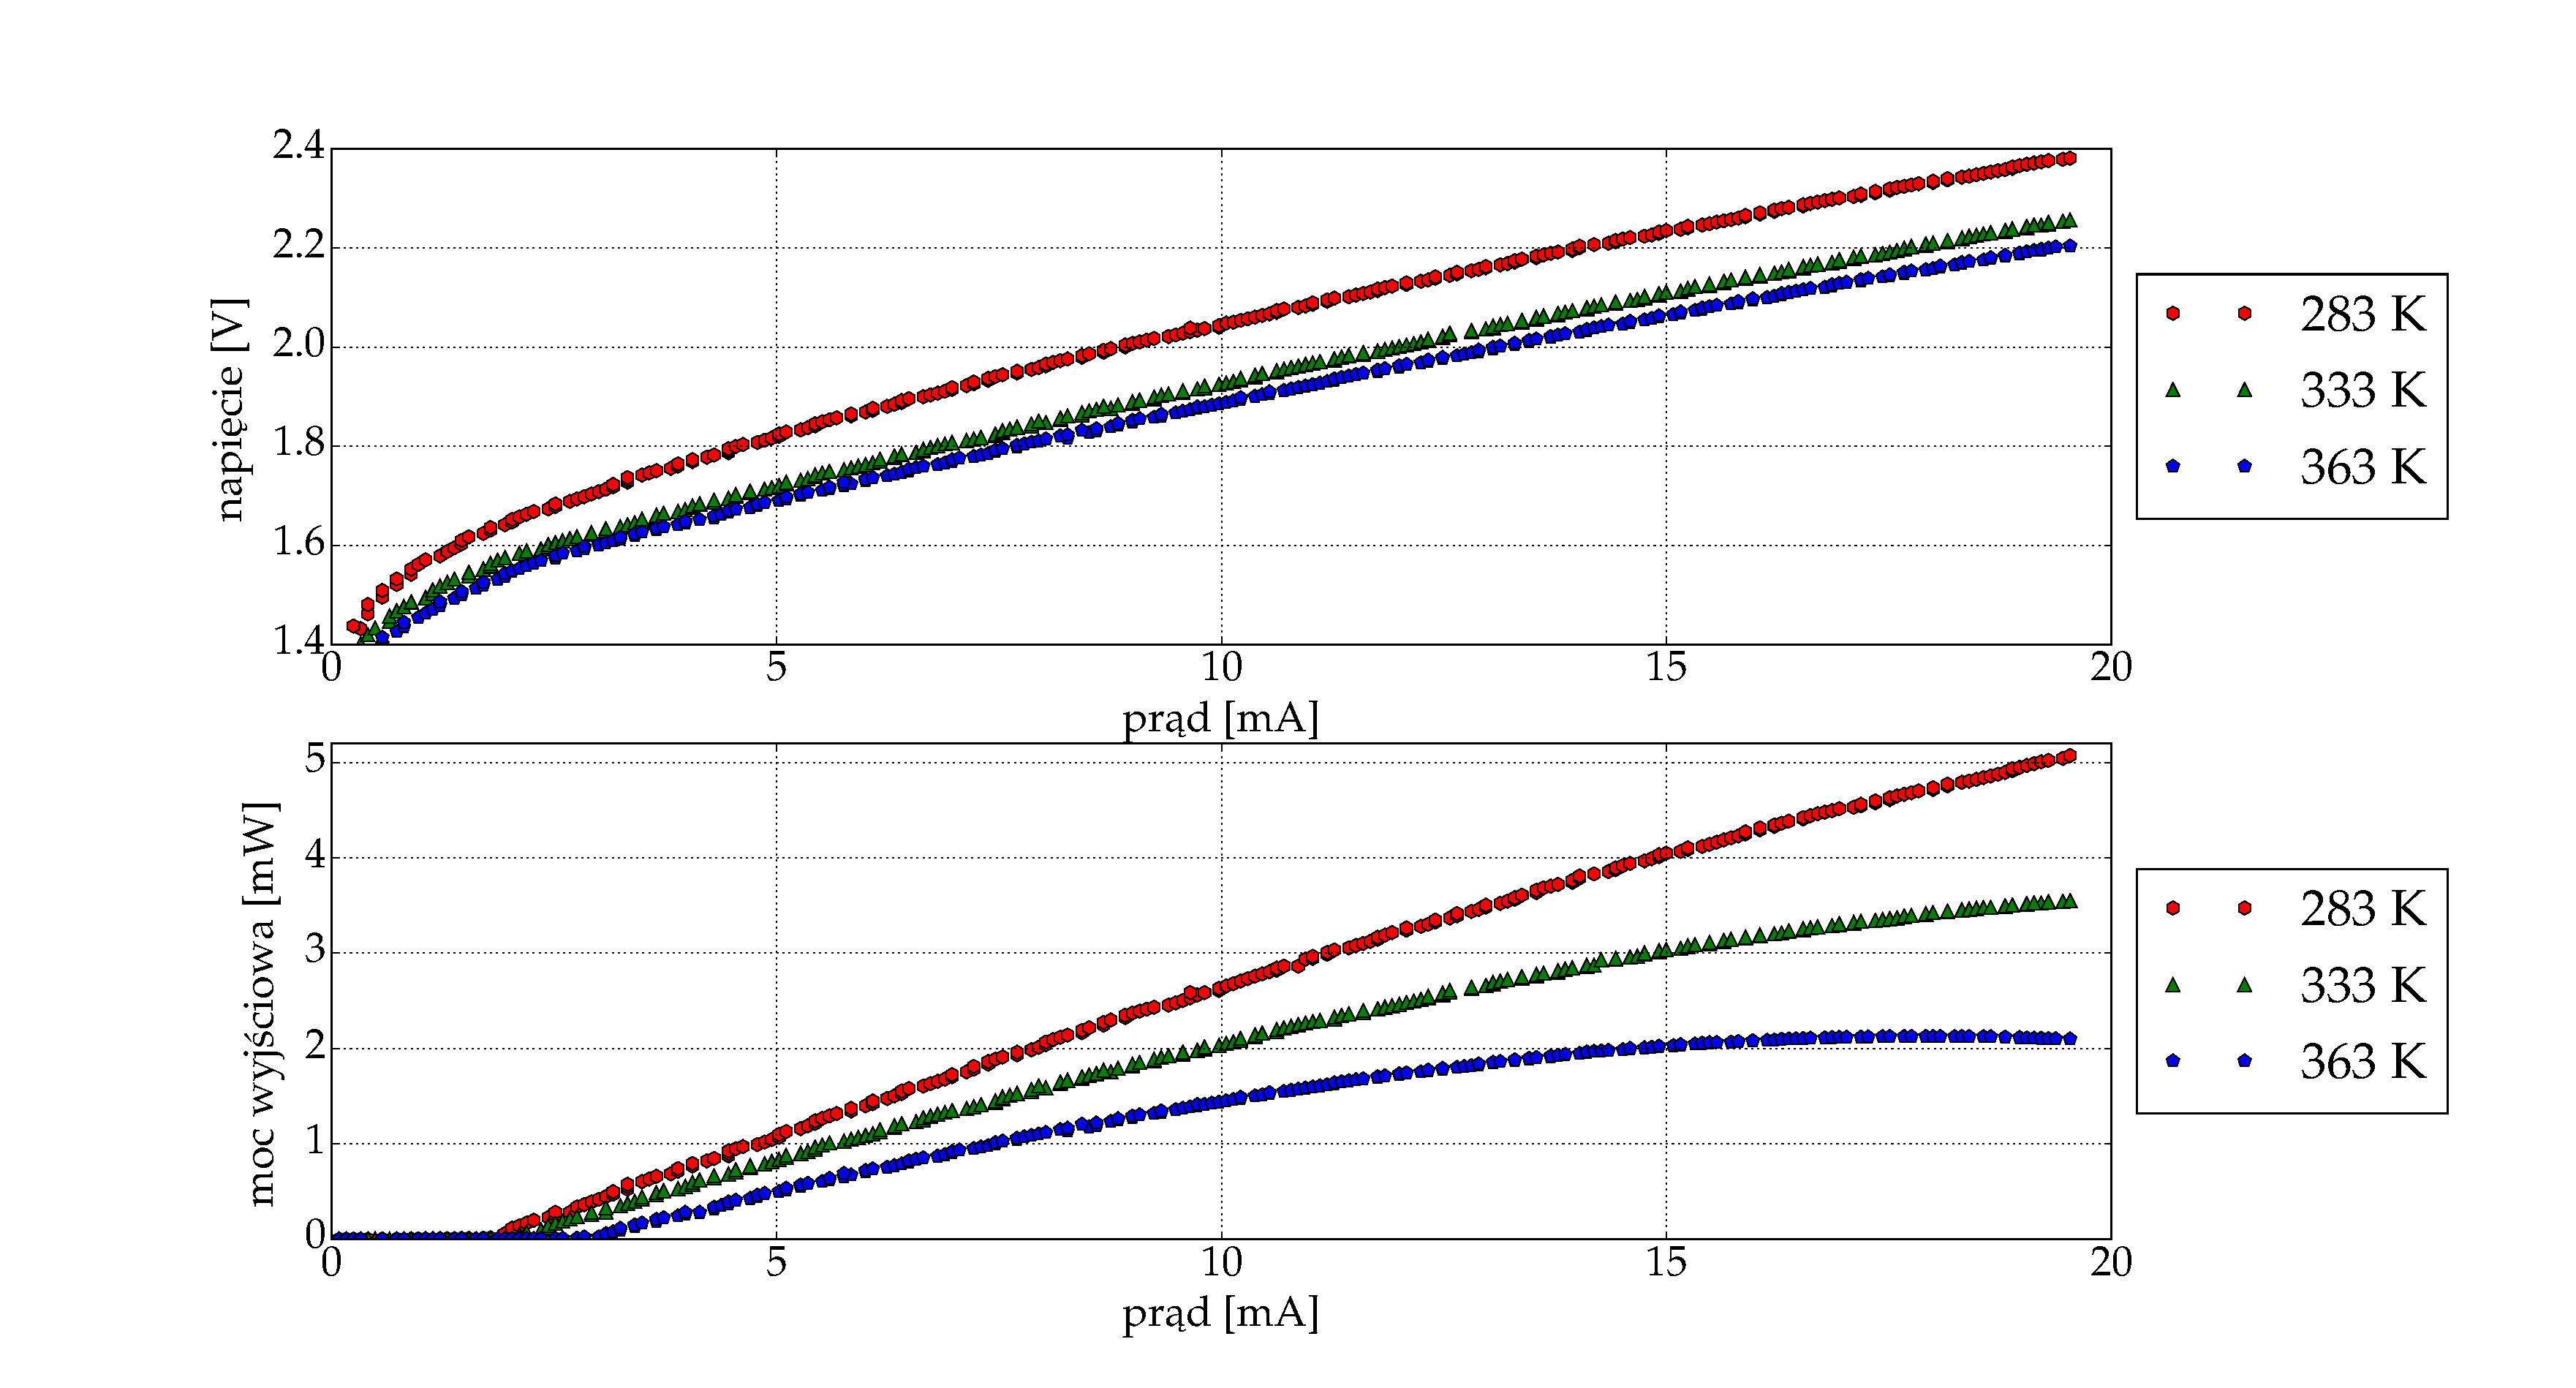
\includegraphics[scale=0.30]{plot_vcsel_850/plot_power_voltage.eps}
  \caption{Wykres napięcia na laserze i mocy wyjściowej w funkcji prądu od temperatury chłodnicy dla lasera VCSEL 850\,nm.}
  \label{fig:plot_power_voltage_vcsel850}
\end{figure}
%\begin{figure}
%\center
%  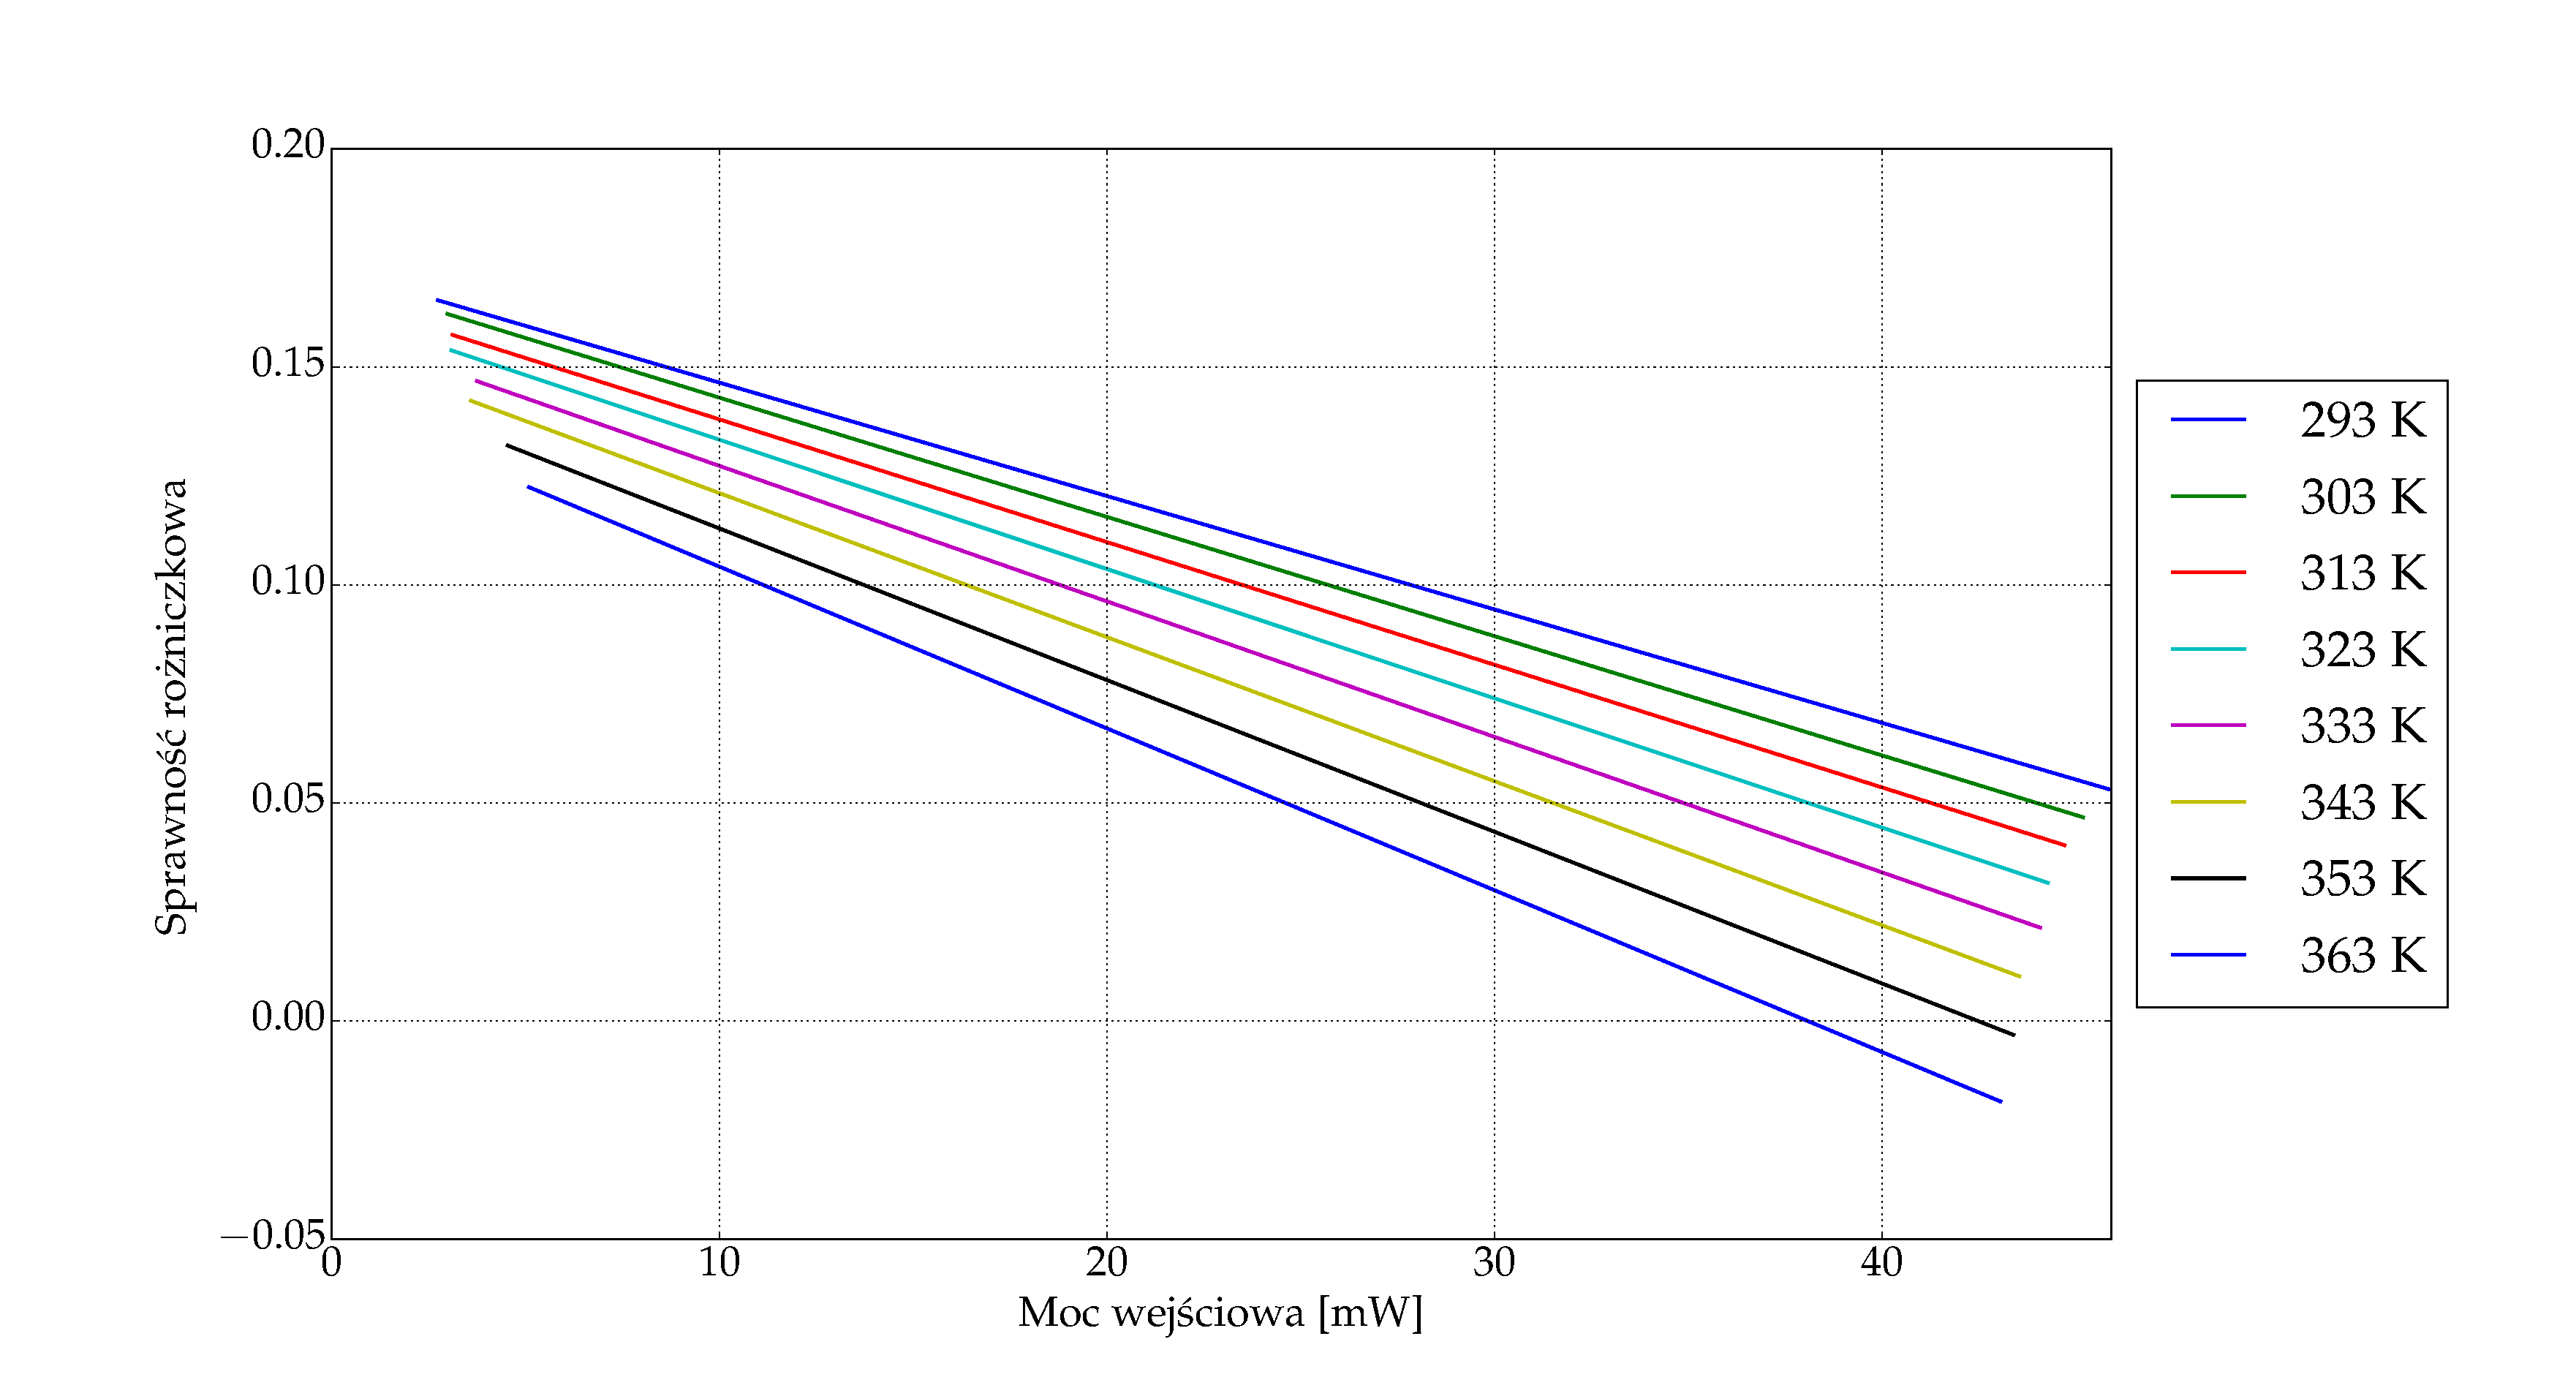
\includegraphics[scale=0.30]{plot_vcsel_850/plot_eff_all_via_power.eps}
%  \caption{Sprawność VCSEL 850 w funkcji mocy wejściowej.}
%  \label{vcsel_850_rys_4}
%\end{figure}
%\begin{figure}
%\center
%  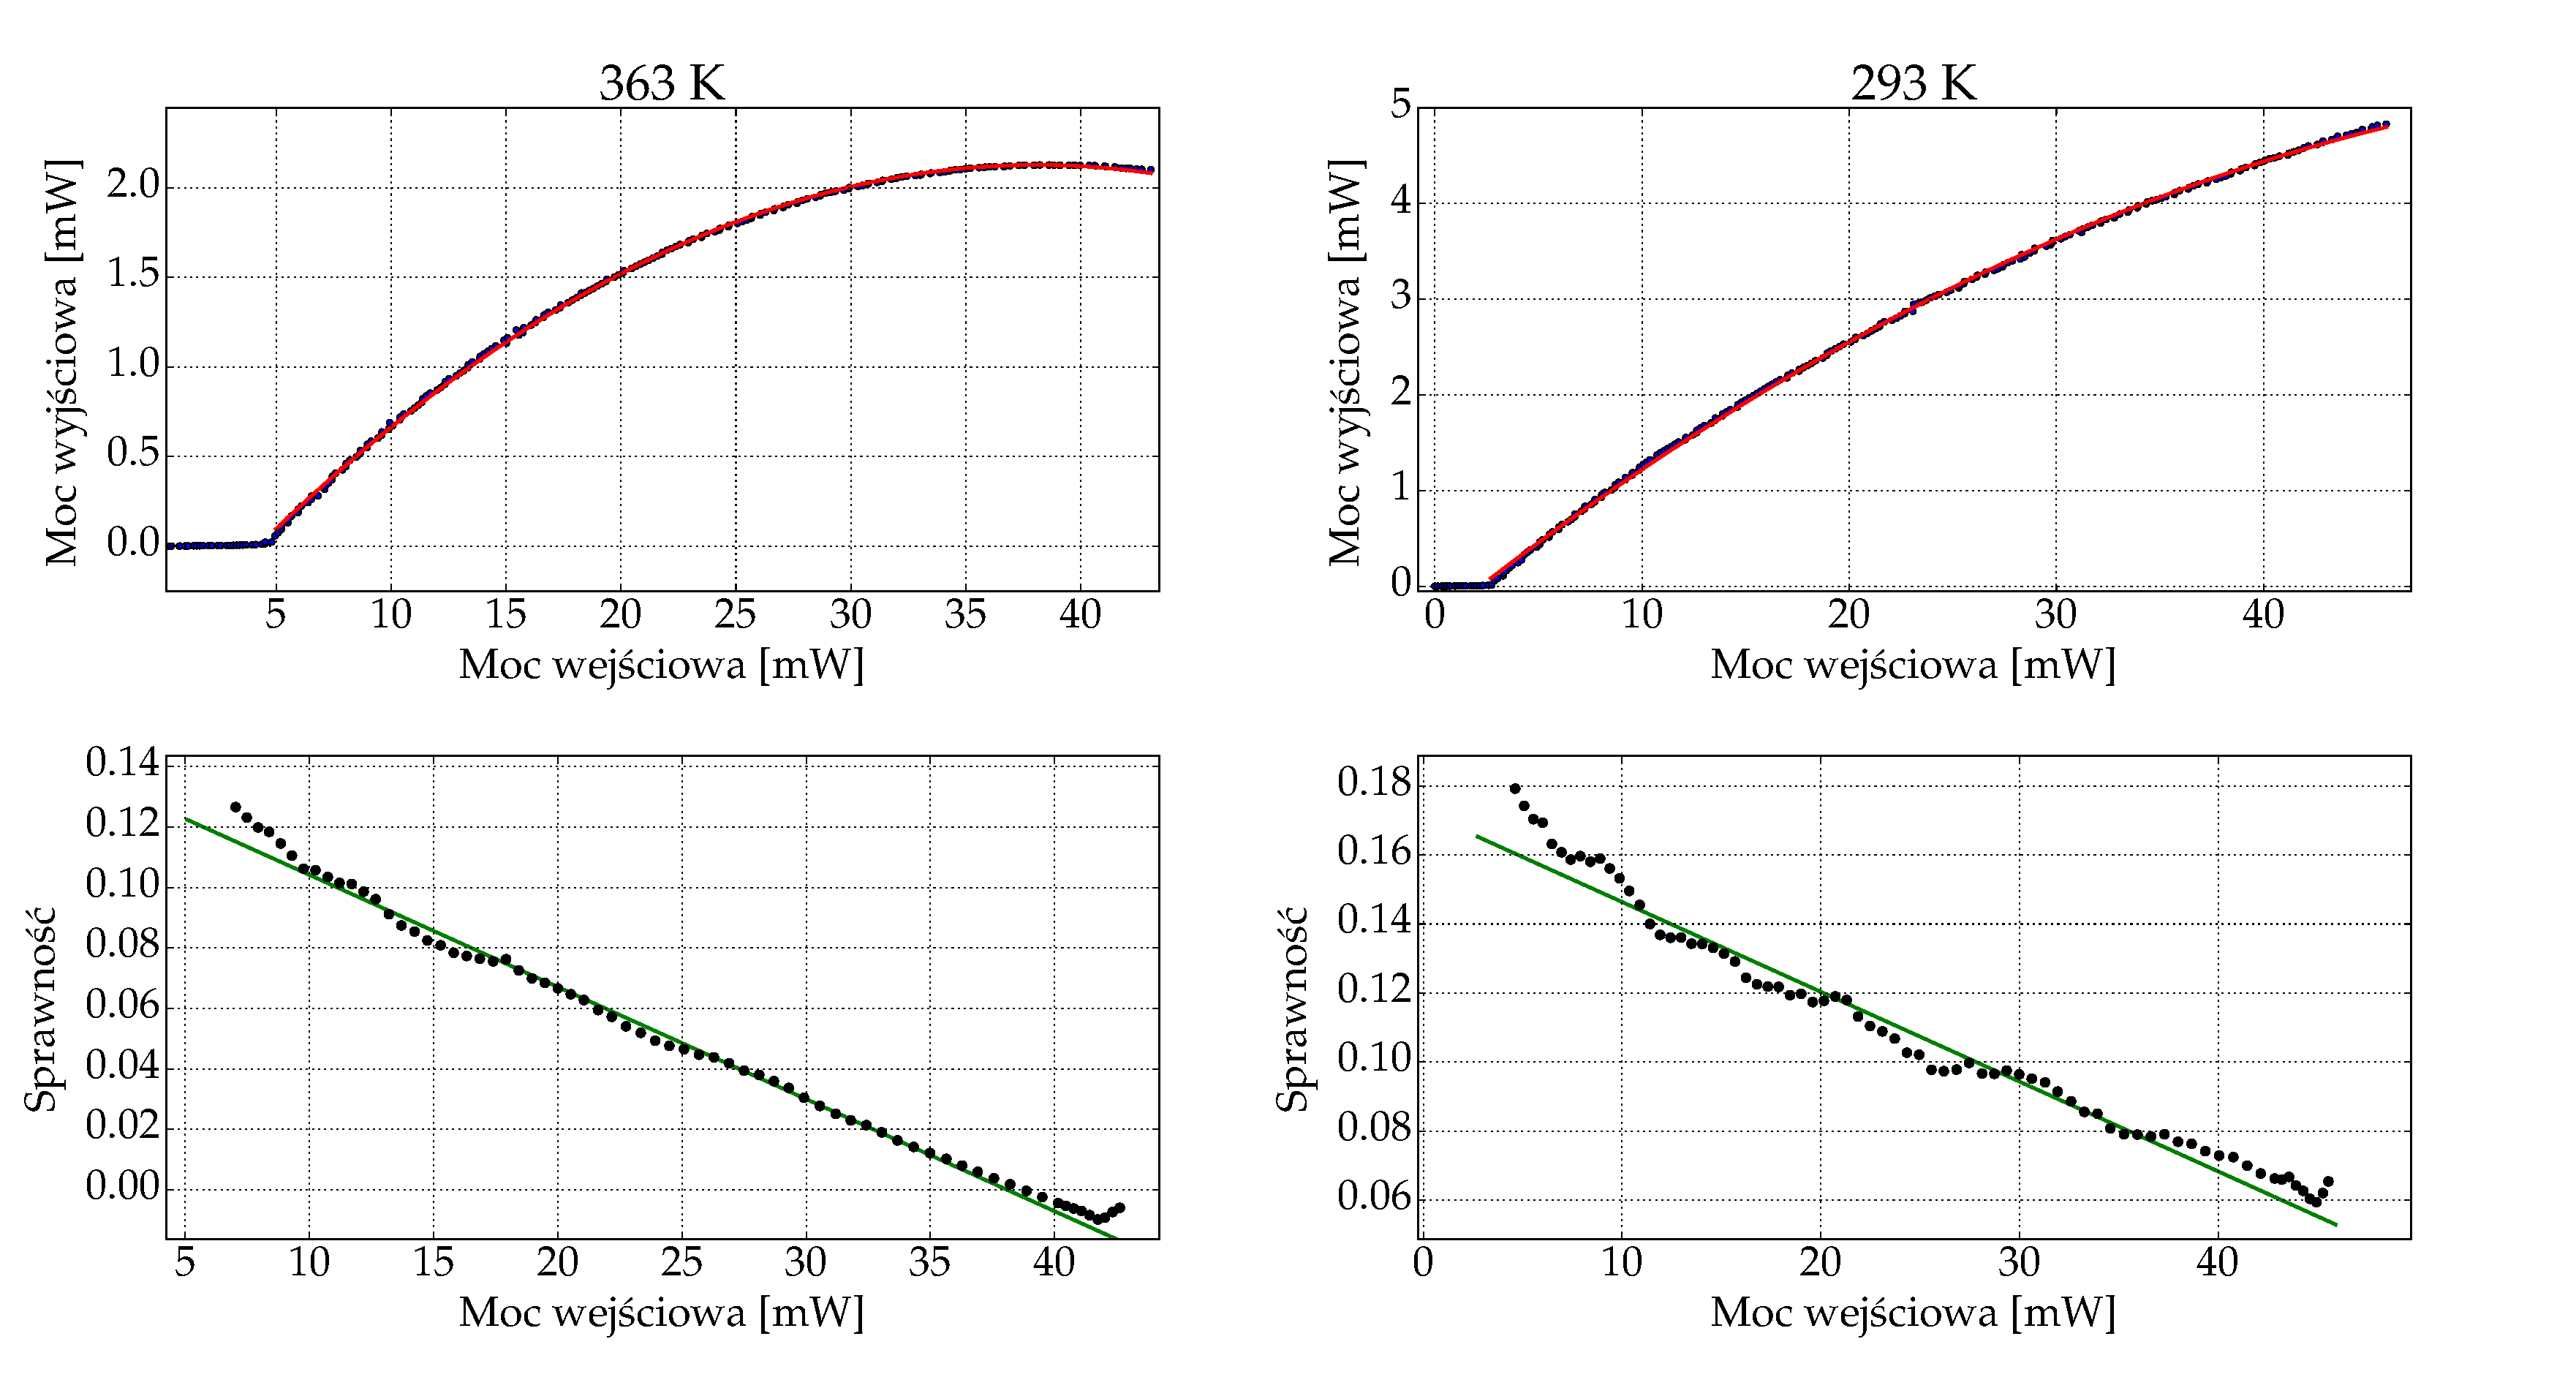
\includegraphics[scale=0.30]{plot_vcsel_850/plot_eff_20_90_via_power.eps}
%  \caption{Sprawność VCSEL 850 dla temperatury 293\,K i 363\,K.}
%  \label{vcsel_850_rys_5}
%\end{figure}
%\begin{figure}
%\center
%  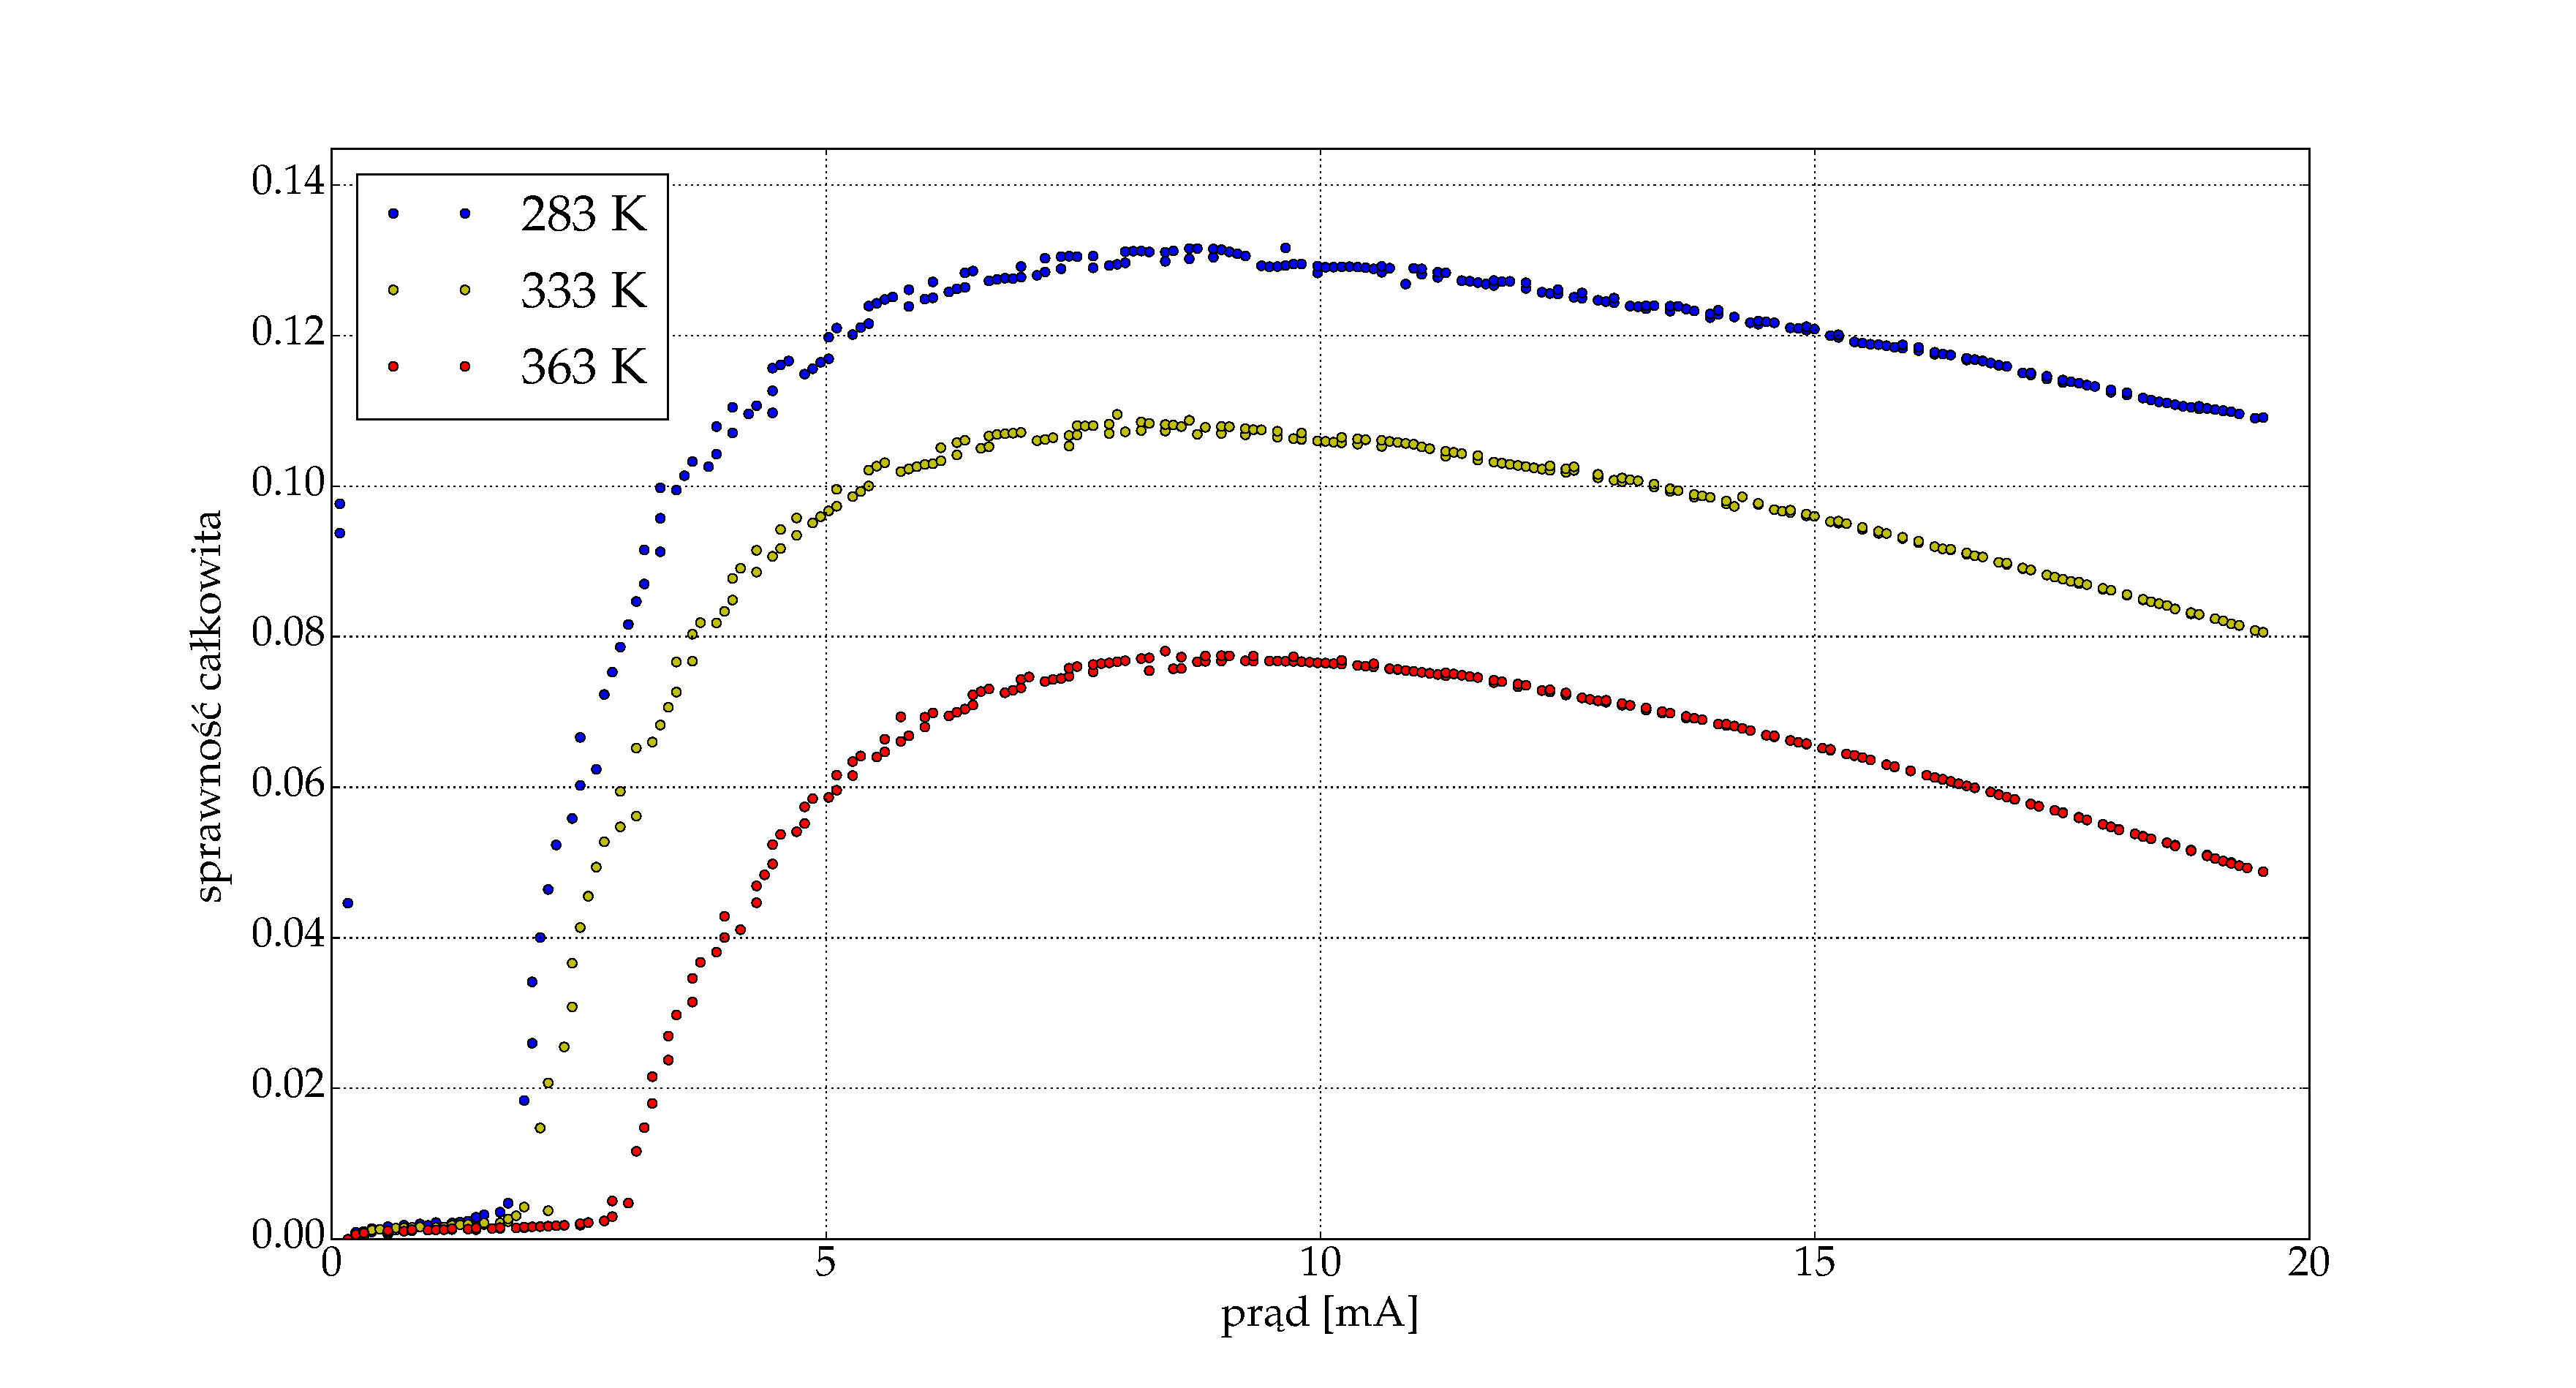
\includegraphics[scale=0.30]{plot_vcsel_850/plot_eff_wall.eps}
%  \caption{Sprawność całkowita dla lasera VCSEL 850\,nm w różnych temperaturach.}
%  \label{vcsel_850_rys_8}
%\end{figure}
\begin{figure}
\center
  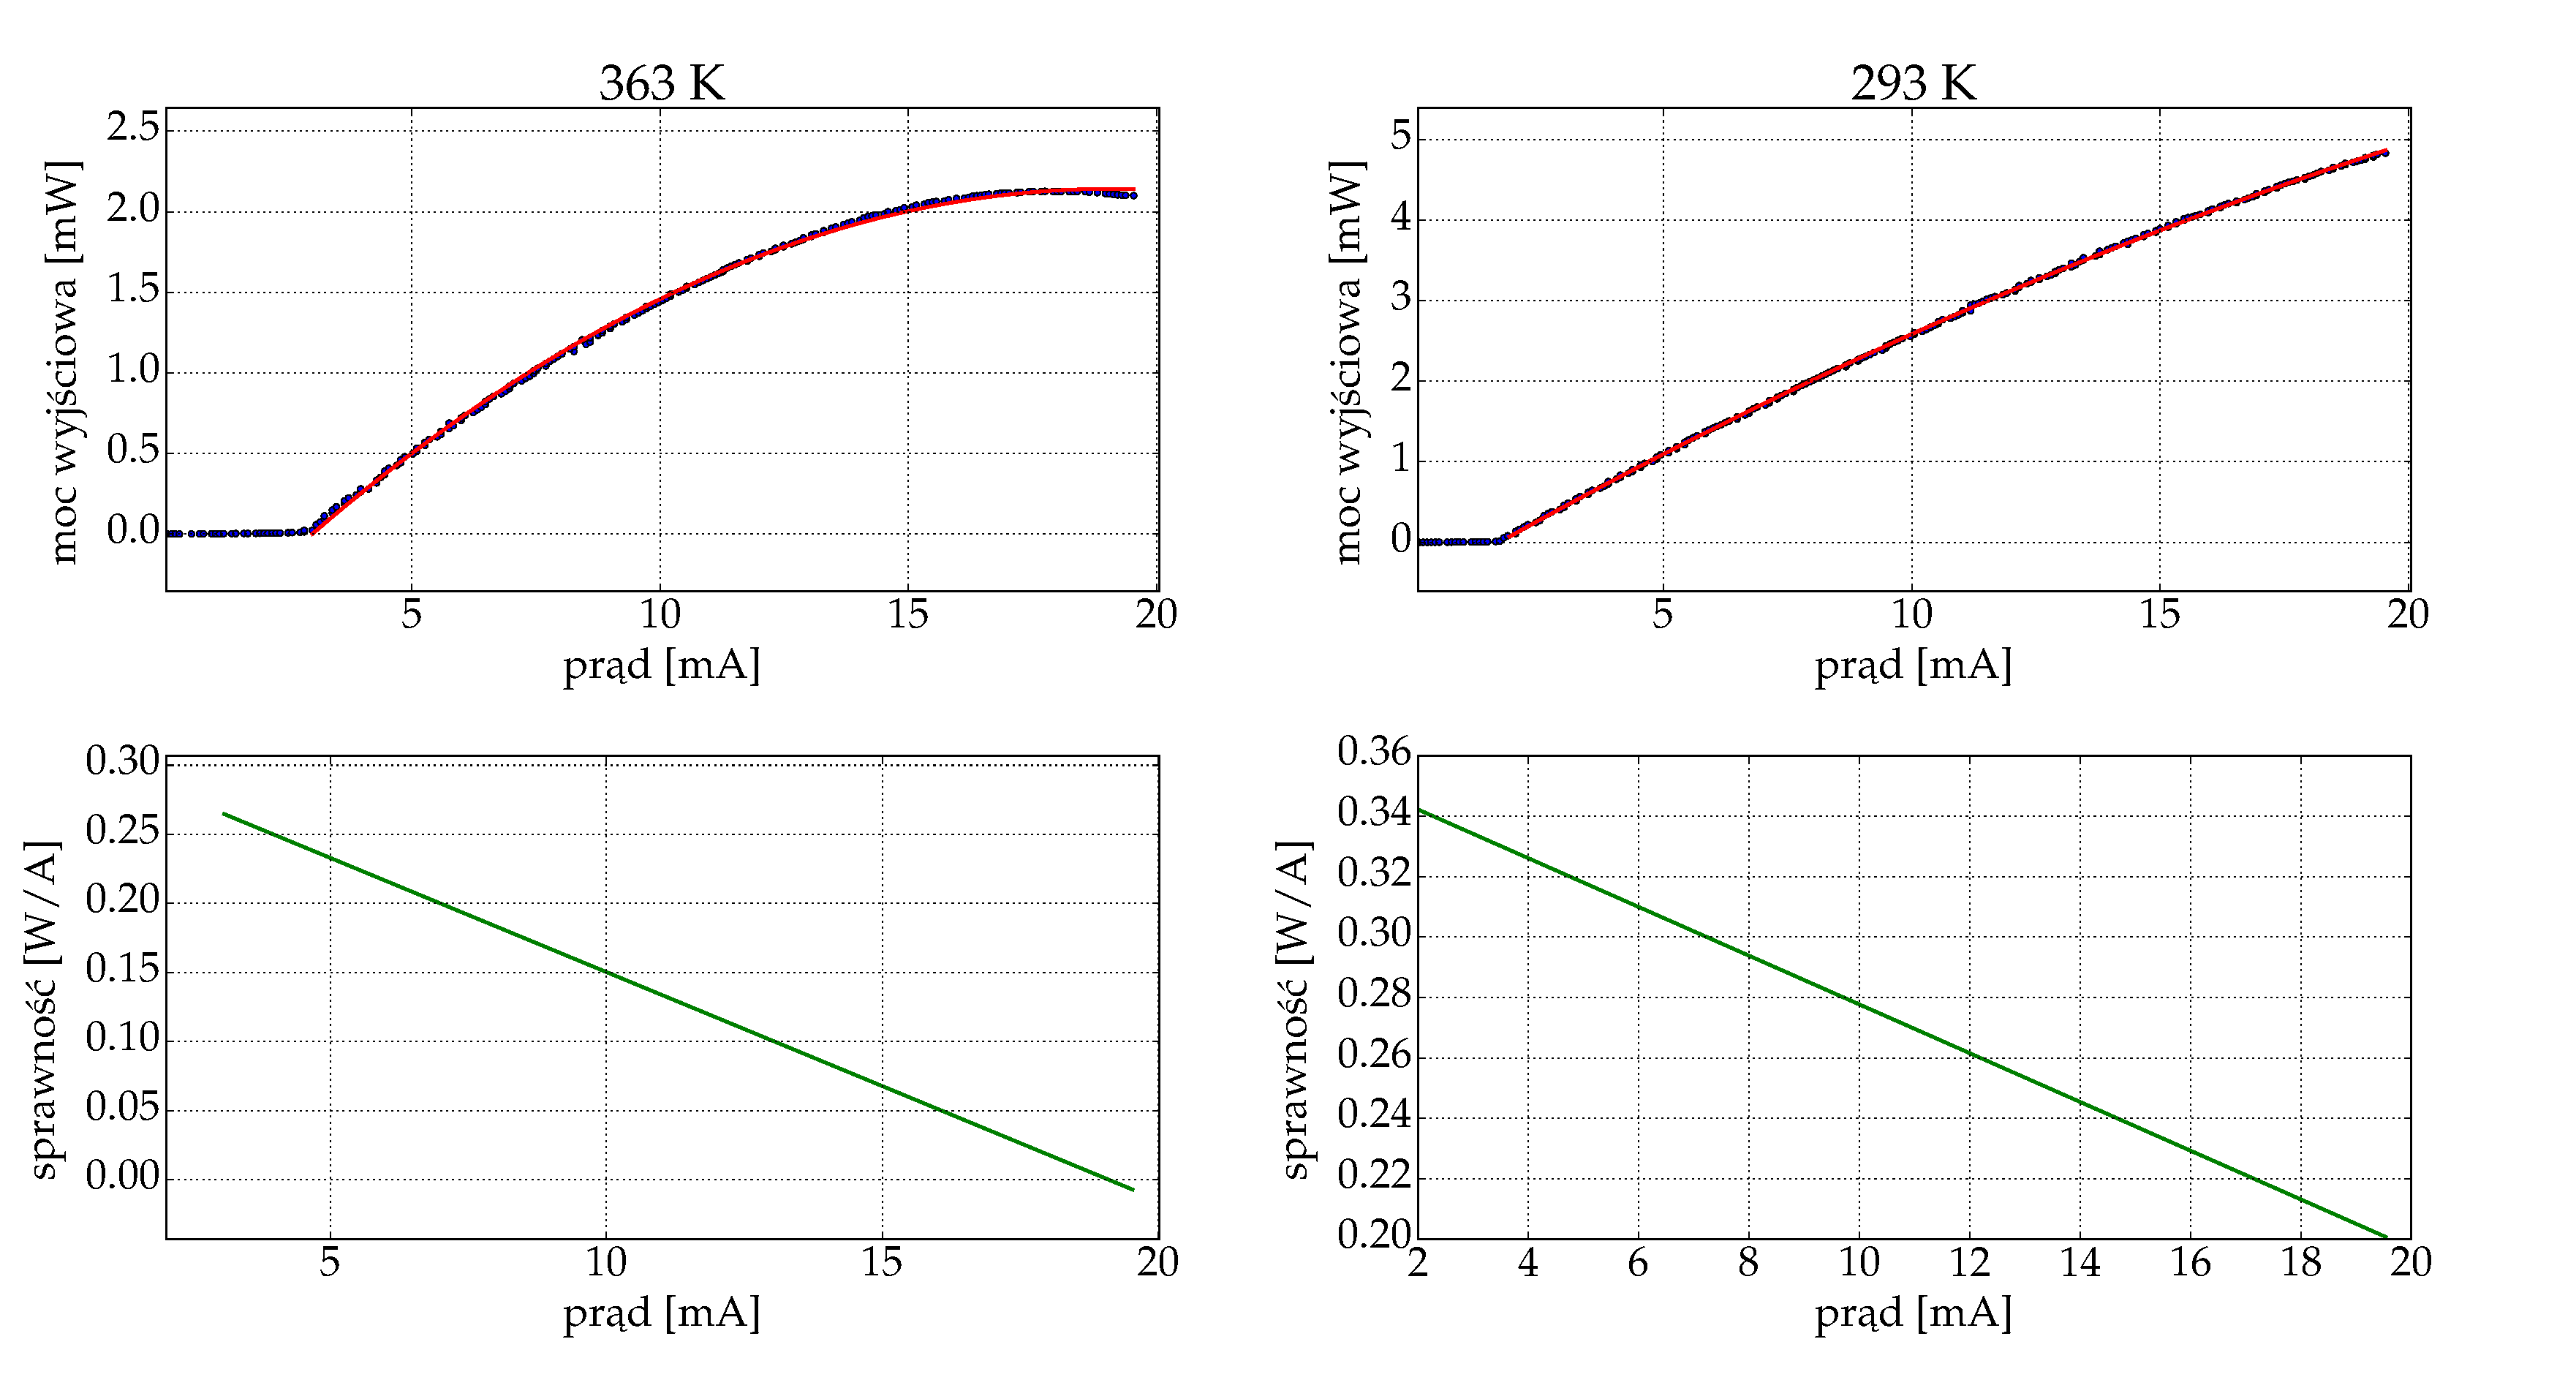
\includegraphics[scale=0.30]{plot_vcsel_850/plot_eff_all_via_current2.eps}
  \caption{Sprawność różniczkowa dla lasera VCSEL 850\,nm w różnych temperaturach.}
  \label{fig:plot_eff_all_via_current2_vcsel850}
\end{figure}
\begin{figure}
\center
  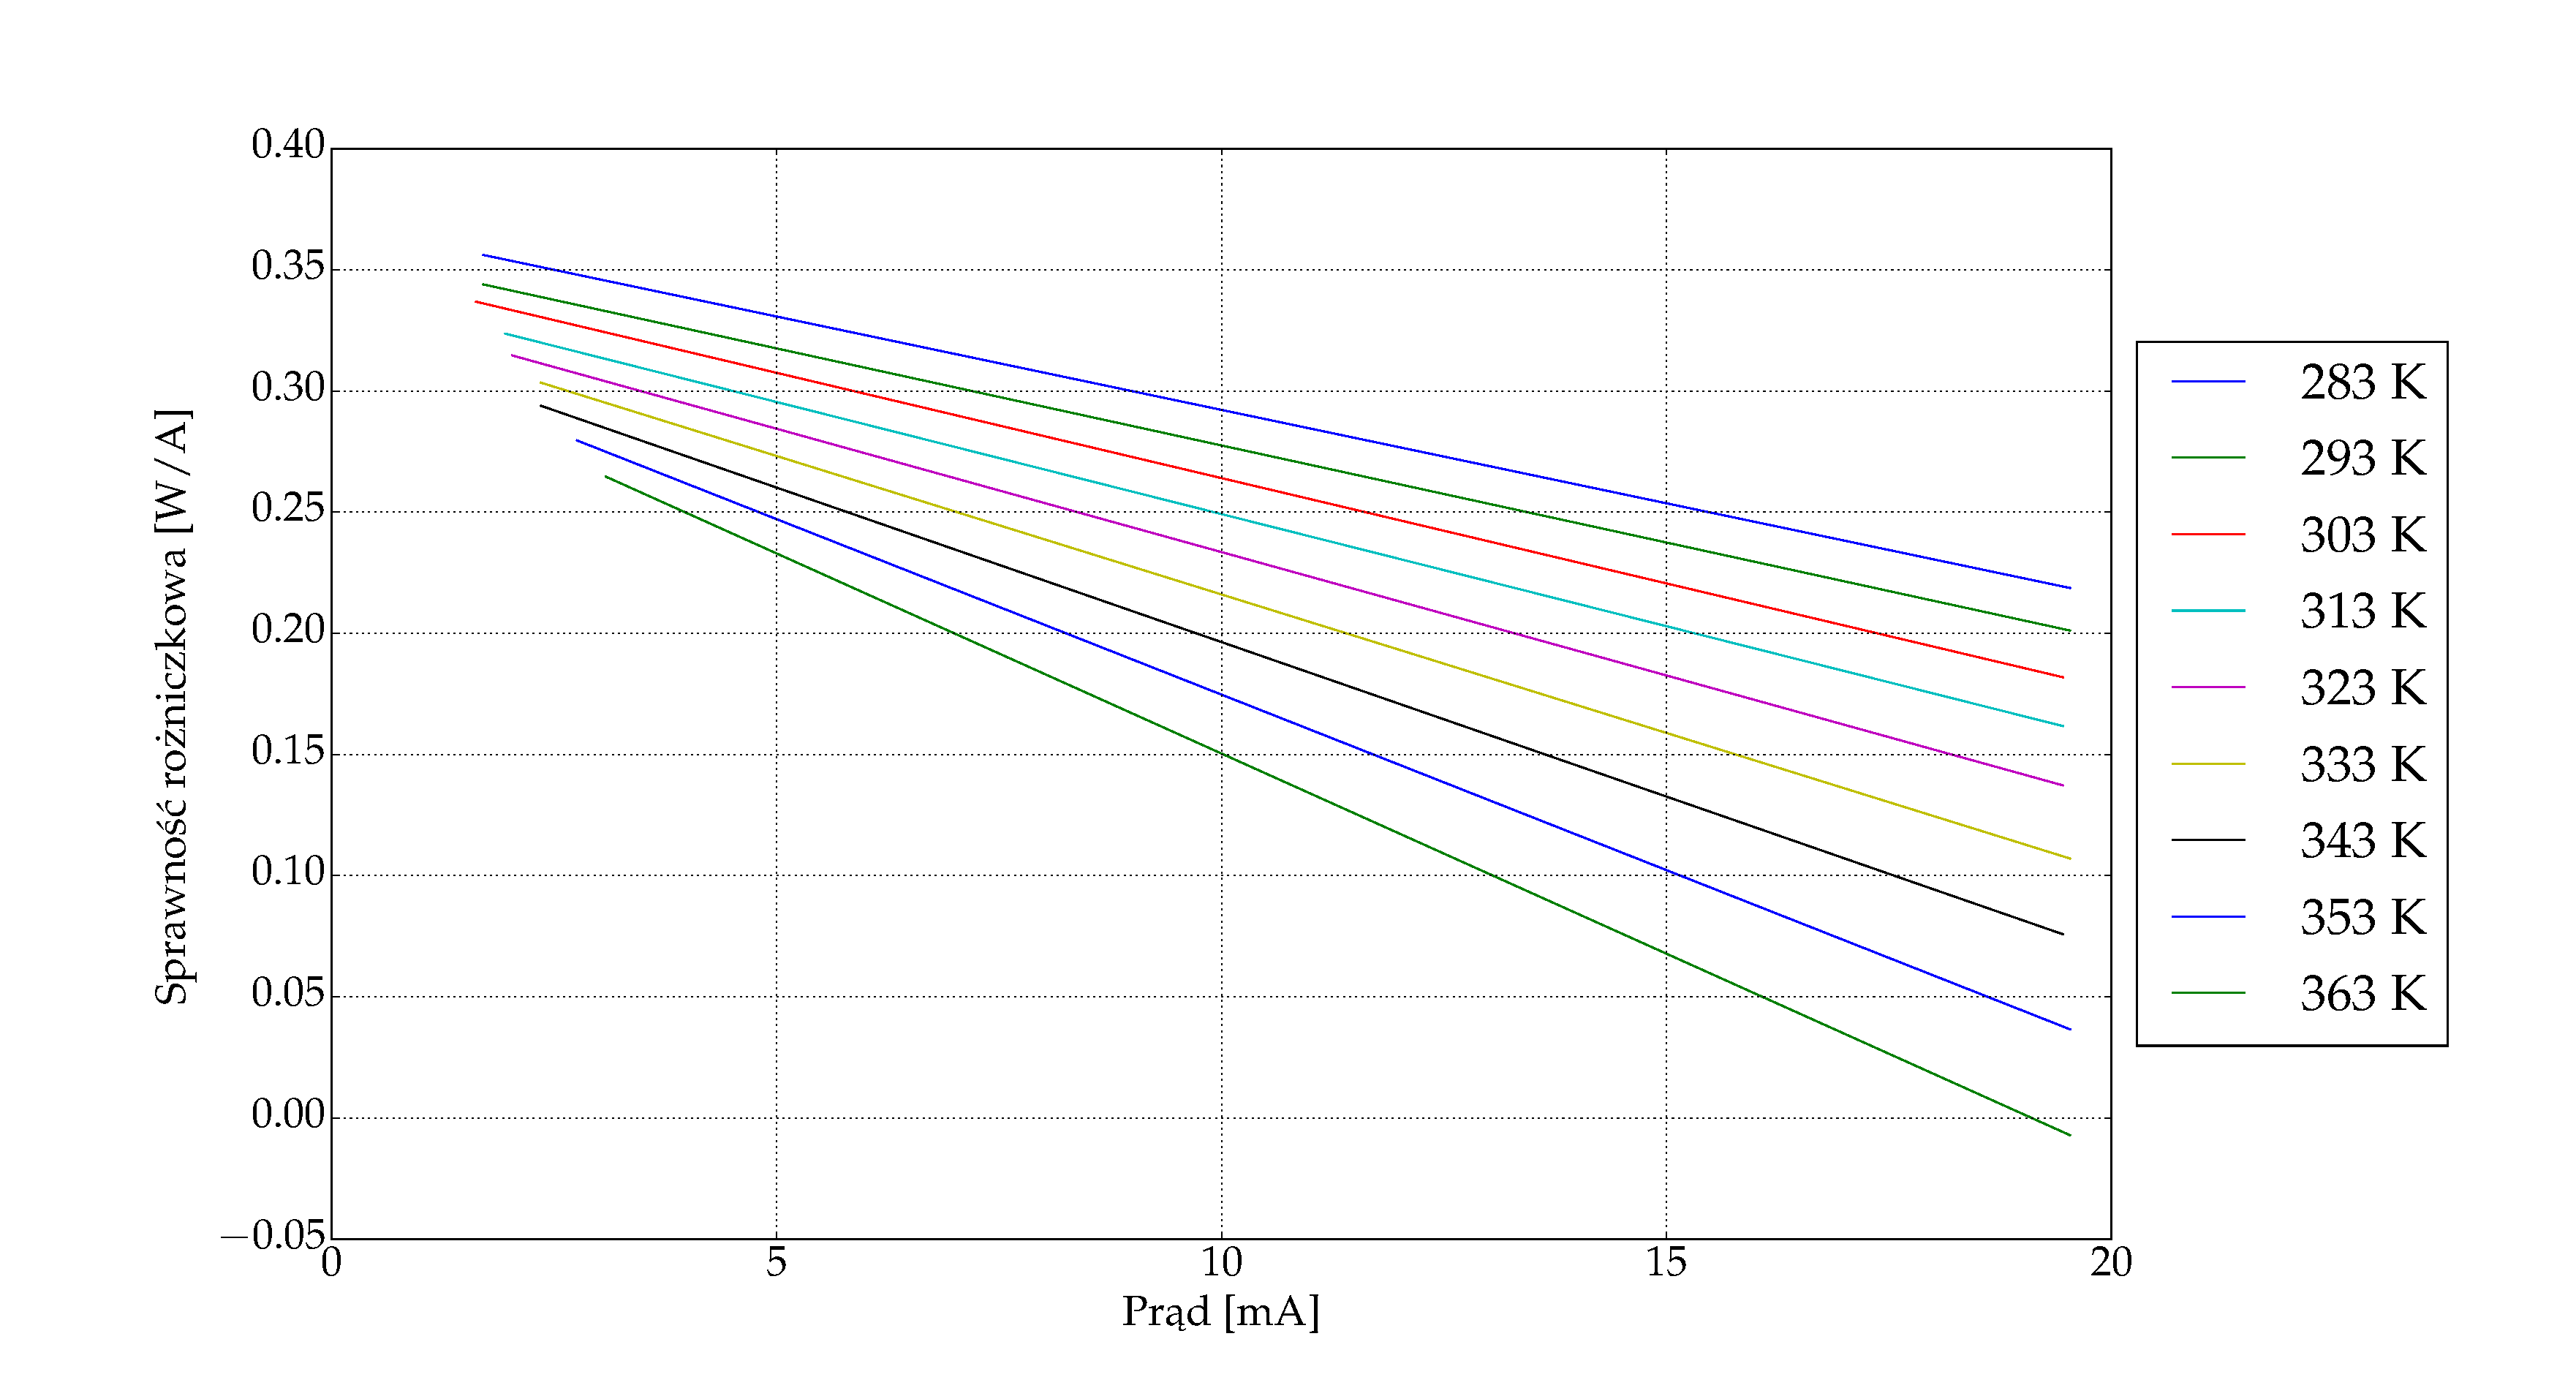
\includegraphics[scale=0.25]{plot_vcsel_850/plot_eff_all_via_current.eps}
  \caption{Sprawność różniczkowa lasera VCSEL 850 w funkcji prądu dla różnych temperatur.}
  \label{fig:plot_eff_all_via_current_vcsel850}
\end{figure}
\newpage
%\section{Omówienie wyników}
%Dzięki analizie sporządzonych wykresów można dojść do następujących konkluzji:
%\begin{itemize}
%\item Analizując wykres napięcia na laserze od prądu wejściowego przedstawiony na rysunku~\ref{vcsel_850_rys_1} oraz~\ref{vcsel_850_rys_2} można zauważyć, że wraz ze wzrostem temperatury na chłodnicy
%maleje opór lasera. Także, wraz z wyższą temperaturą chłodnicy maleje moc wyjściowa lasera.
%\item Wykres na rysunku~\ref{vcsel_850_rys_3} przedstawia sprawność różniczkowa lasera w funkcji prądu wejściowego od temperatury na chłodnicy, jak wynika z wykresu im
%wyższa temperatura tym sprawność lasera mniejsza.
%\item Wykres na rysunku~\ref{vcsel_850_rys_4} przedstawia sprawność różniczkowa lasera w funkcji mocy wejściowej od temperatury na chłodnicy, jak wynika z wykresu im
%wyższa temperatura tym sprawność lasera mniejsza.
%\item Wykres na rysunku~\ref{vcsel_850_rys_5} przedstawia w górnej cześci zależności mocy wyjściowej od mocy wejściowej.
%\item Wykres na rysunku~\ref{vcsel_850_rys_7} pokazuje zależności prądu progowego od temperatury. Jak widzimy przy temperaturach (280-300)\,K
%wraz ze wzrostem temperatury maleje wartość prądu progowego, natomiast dla temperatur $>$ 300\,K im wyższa temperatura to zwiększa się
%wartość prądu progowego.
%\item Wykres na rysunku~\ref{vcsel_850_rys_8} przedstawia sprawnośc całkowitą lasera dla trzech temperatur: 283\,K, 333\,K, 363\,K. Analizując ten wykres
%dochodzę do wniosku, że im wyższa temperatura tym sprawnośc mniejsza.
%\item Wykres na rysunku~\ref{vcsel_850_rys_9} przedstawia sprawności różniczkowe dla dwóch temperatur. W górnej cześci przedstawiona jest charakterystyka
%wyjściowa z dopasawaną funkcją w postaci wielomianu stopnia drugiego. Pochodna tej funkcji jest sprawnością rożniczkową. Na dolnym wykresie przedstawiona
%jest sprawność w postaci prostej będącej pochodną dopasowanej funkcji. Natomiast czarne kropki przedstawiają sprawność powstałą w wyniku obliczenia pochylenia
%10 punktów przefiltrowanych co 3 punkty.
%\end{itemize}

\end{document}
\grid
